\documentclass[11pt,a4paper]{ctexart}
\usepackage{amsthm, amssymb, graphicx,mathrsfs,amsmath}
\usepackage{geometry}
\usepackage[colorlinks=true,hidelinks]{hyperref} % 目录添加超链接
\geometry{left=1.24cm, right=1.24cm, top=1.91cm, bottom=1.91cm}
\title{随机控制理论}
\author{W·D·Gaster}
\renewcommand{\d}{{\rm d}}
\newcommand{\e}{{\rm e}}
\renewcommand{\j}{{\rm j}}
\usepackage{booktabs}
\usepackage{pifont} %使用带圈数字序号
\usepackage{enumitem} %自定义列表序号
\usepackage{bm}

\graphicspath{{figures/}} % 指定图片路径
\usepackage{float}

\begin{document}

\maketitle
\thispagestyle{empty}
\newpage

\tableofcontents
\thispagestyle{empty}
\newpage

\setcounter{page}{1}
\section{随机过程}
    随机事件的样本空间$\Omega=\{\omega\}$，有确定的时间函数$X(t,\omega),t\in T$与之对应，则对所有$\omega\in\Omega$，得到一组$t$的函数成为随机过程，每一个确定的函数称为样本函数。
    对于每一个特定时间$t_i$，$X(t_i,\omega)$为一组随机变量，则$X(t,\omega)$为随机过程，$X(t_i,\omega)$为在$t_i$时刻的状态。

    根据连续性，随机过程分为：
    \begin{itemize}
        \item 连续型随机过程：$t$连续且$X(t_i,\omega)$为连续随机变量；
        \item 离散型随机过程：$t$连续且$X(t_i,\omega)$为离散随机变量；
        \item 连续型随机序列：$t$离散且$X(t_i,\omega)$为连续随机变量；
        \item 离散型随机序列：$t$离散且$X(t_i,\omega)$为离散随机变量。
    \end{itemize}

    $X(t)$在$t_i\in T$取值为n维随机变量
    \[
    F_x(x_1,x_2,\cdots,x_n;t_1,t_2,\cdots,t_n)=P(X(t_1)\leqslant x_1;X(t_2)\leqslant x_2;\cdots;X(t_n)\leqslant x_n)
    \]
    
    若$t_i$为任意值则为n维分布函数族，若偏导存在，则n维概率密度
    \[
    f_x(x_1,x_2,\cdots,x_n;t_1,t_2,\cdots,t_n)=\dfrac{\partial F_x(x_1,x_2,\cdots,x_n;t_1,t_2,\cdots,t_n)}{\partial x_1\partial x_2\cdots\partial x_n}
    \]
    \subsection{随机过程的数字特征}
        \paragraph{数学期望}\leavevmode

        对于一维，$m_x(t)=E\{X(t)\}=\int_{-\infty}^{\infty}xf(x;t)\d x$；
        
        对于n维，
        \[
        E\{\bm{X}(t)\}=[E\{X_1(t)\},E\{X_2(t)\},\cdots,E\{X_n(t)\}]^T
        \]

        \paragraph{方差}\leavevmode
        
        对于一维，$R_x(t)=Var\{X(t)\}=E\{(x-m_x(t))^2\}$；
        
        对于n维，$R_{x_i}(t)$为方差，$R_{x_ix_j}(t)$为协方差，
        \[
        R_x(t)=\begin{bmatrix}R_{x_1}(t)&R_{x_1x_2}(t)&\cdots&R_{x_1x_n}(t)\\R_{x_2x_1}(t)&R_{x_2}(t)&\cdots&R_{x_2x_n}(t)\\\vdots&\vdots&\ddots&\vdots\\R_{x_nx_1}(t)&R_{x_nx_2}(t)&\cdots&R_{x_n}(t)\end{bmatrix}
        \]

        \paragraph{自相关函数}\leavevmode
        
        $C_x(t_1,t_2)=E\{X(t_1)X(t_2)\}$，描述两时刻间的状态关系

        \paragraph{自协方差函数}\leavevmode
        
        $R_x(t_1,t_2)=E\{[x(t_1)-m_x(t_1)][x(t_2)-m_x(t_2)]\}$，描述两时刻间的状态波动相关性。
    \subsection{随机过程的性质}
        \paragraph{平稳性}\leavevmode
        
        $f(x_1,x_2,\cdots,x_n)$中，当$x_1\rightarrow x_1+\Delta x_1$时，$f(x_1+\Delta x_1,x_2,\cdots,x_n)$特性不变（对于确定函数函数值不变，对于随机过程统计特性不变），则$f$关于$x_1$平稳。

        严平稳随机过程（窄平稳，强平稳）：$\forall t_i,t_i+\tau\in T,\tau\in\mathbb{R}$，满足$f_x(x_1,t_1;x_2,t_2;\cdots;x_n,t_n)=f_x(x_1,t_1+\tau;x_2,t_2+\tau;\cdots;x_n,t_n+\tau)$，均值和方差与时间无关，自相关函数和自协方差函数是时间差的函数。

        宽平稳随机过程（弱平稳，二阶平稳）：$m_x(t)=m_x,R_x(t_1,t_2)=R_x(t),E\{x^2(t)\}<\infty$，二阶矩有限的严平稳过程必定是宽平稳过程，宽平稳过程不一定是严平稳过程。

        协方差平稳过程：$r(t,t+\tau)=r(\tau)$，协方差函数仅是时差的函数。

        \paragraph{遍历性（各态历经性）}\leavevmode
        
        随机过程的统计平均（总体平均）几乎处处可以由一个样本函数的时间平均来描述，设$f(x)$为随机过程的一个已知函数，$\lim\limits_{T\rightarrow\infty}\dfrac{1}{2T}\int_{-T}^{T}f(X(t))\d t \overset{a.s.}{=}E\{f(X(t))\}$。

        严遍历（强遍历）：各时间平均几乎处处收敛于相应统计平均。
        
        宽遍历（弱遍历）：均值与相关函数有遍历性。

        $f(x(t))=x(t)$时，$\lim\limits_{T\rightarrow\infty}\dfrac{1}{2T}\int_{-T}^{T}x(t)\d t \overset{a.s.}{=}E\{X(t)\}$，称为均值遍历性；

        $f(x(t))=x^2(t)$时，$\lim\limits_{T\rightarrow\infty}\dfrac{1}{2T}\int_{-T}^{T}x^2(t)\d t \overset{a.s.}{=}E\{X^2(t)\}$，称为均方遍历性；

        $f(x(t))=x(t)x(t+\tau)$时，$\lim\limits_{T\rightarrow\infty}\dfrac{1}{2T}\int_{-T}^{T}x(t)x(t+\tau)\d t \overset{a.s.}{=}E\{X(t)X(t+\tau)\}=\varGamma(\tau)=C_x(t,t+\tau)$，称为相关遍历性。

        均值遍历仅当$\lim\limits_{T\rightarrow\infty}\dfrac{1}{T}\int_{0}^{2T}\left(1-\dfrac{\tau}{2T}\right)[\varGamma(\tau)-m^2]\d\tau=0$

        相关函数遍历仅当$\lim\limits_{T\rightarrow\infty}\dfrac{1}{T}\int_{0}^{2T}\left(1-\dfrac{\tau_1}{2T}\right)[\xi(\tau_1)-\varGamma^2(\tau)]\d\tau_1=0$，其中$\xi(\tau_1)=E\{x(t+\tau+\tau_1)x(t+\tau_1)x(t+\tau)x(t)\}$

        随机过程遍历一定是相同意义下平稳的，但平稳过程不一定是各态遍历的。
    \subsection{随机积分}
        \subsubsection{均方微积分}
            随机过程$\{x(t),t\in T\}$对所有的$t\in T$都存在均方值，即$E\{x^2(t)\}<\infty,\forall t\in T$，则称为二阶矩过程。由Schwarz不等式可知均值和协方差函数一定存在。在均方极限意义下二阶矩过程的随机分析即为均方微积分。

            \paragraph{均方极限}\leavevmode

            如有$\lim\limits_{n\rightarrow\infty}d(x_n,x)=\lim\limits_{n\rightarrow\infty}\|x_n-x\|=0$，则称$x_n$均方收敛于$x$，记作$\lim\limits_{n\rightarrow\infty}x_n=x$

            均方收敛准则：充要条件是$\lim\limits_{m,n\rightarrow\infty}E\{x_mx_n\}=\lim\limits_{m,n\rightarrow\infty}(x_m,x_n)=c$，此时有$\lim\limits_{n\rightarrow\infty}E\{x_mx_n\}=E\{x^2\}=\|x\|^2$
            \paragraph{均方极限的性质}
            \begin{itemize}
                \item $\lim\limits_{n\rightarrow\infty}E\{x_n\}=E\{\lim\limits_{n\rightarrow\infty}x_n\}=E\{x\}$，均方极限和期望运算可交换
                \item $\lim\limits_{m,n\rightarrow\infty}(x_m,y_n)=(x,y)=\lim\limits_{m,n\rightarrow\infty}E\{x_my_n\}=E\{xy\}$
                \item 满足线性运算，$\lim\limits_{n\rightarrow\infty}(ax_n+by_n)=ax+by$
                \item 均方极限是唯一的，即若$\lim\limits_{n\rightarrow\infty}x_n=x,\lim\limits_{n\rightarrow\infty}y_n=y$，则$x=y$
            \end{itemize}

            \paragraph{均方连续}\leavevmode

            如有$\lim\limits_{t\rightarrow t_0}\|x(t)-x(t_0)\|=0$，则称在$t_0$均方连续，若对一切$t\in T$都成立，则称在$T$上均方连续。

            均方连续准则：充要条件是均值函数$m(t)$在$t$处连续和自协方差函数$Cov(x(t),x(\tau))$在$(t,t)$处连续，等价为自相关函数$\varGamma(t,\tau)=Cov(x(t),x(\tau))+m(t)m(\tau)$在$(t,t)$处连续。

            \paragraph{均方可微}\leavevmode

            如有$\lim\limits_{\tau\rightarrow0}\dfrac{x(t+\tau)-x(t)}{\tau}=\dot x(t)$存在，则称均方可微，$\dot x(t)$为均方导数。

            均方可微准则，充要条件是均值函数均方可微且子协方差函数广义二次可微，等价为自相关函数广义二阶导数存在。

            广义二次可微即$\lim\limits_{h,k\rightarrow0}\dfrac{r(t+h,\tau+k)-r(t+h,\tau)-r(t,\tau+k)+r(t,\tau)}{hk}=\dfrac{\partial^2}{\partial t\partial\tau}r(t,\tau)$存在。

            \paragraph{均方导数的性质}
            \begin{itemize}
                \item 在$t$处均方可微则在$t$处均方连续
                \item 均方导数是唯一的，若$\dot x(t)=X,\dot x(t)=Y$，则$X=Y$
                \item 线性性质，$\dfrac{\d}{\d t}[ax(t)+by(t)]=a\dot x(t)+b\dot y(t)$
                \item 乘法性质，$\dfrac{\d}{\d t}[x(t)y(t)]=\dfrac{\d x(t)}{\d t}y(t)+x(t)\dfrac{\d y(t)}{\d t}$
                \item 若n次均方可微，则各均方导数均值存在，且$E\{\dfrac{\d^nx(t)}{\d t^n}\}=\dfrac{\d^n}{\d t^n}E\{x(t)\}$，均方求导和期望可交换
                \item 对宽平稳过程，$r(t,s)=r(t-s)=r(\tau)$，则$\dfrac{\partial^2}{\partial t\partial s}r(t,s)=\dfrac{\partial}{\partial t}\dfrac{\partial}{\partial s}r(t-s)=-\dfrac{\d^2}{\d \tau^2}r(\tau)$，宽平稳过程的均方导数也是宽平稳过程。
            \end{itemize}

            \paragraph{均方积分}\leavevmode

            有$[a,b]\in T$，划分使得$a=t_0<t_1<\cdots<t_n=b,\Delta_n=\max_{k}(t_n-t_{n-1})$，设$t'(k)$是$[t_{k-1},t_k]$内任意一点，如果当$\Delta_n\rightarrow$时有$I_n=\sum\limits_{k=1}^{n}f(t'_k)x(t'(k))(t_k-t_{k-1})$均方收敛且与划分和取法无关，则称黎曼均方可积，极限为黎曼均方积分，记作$I=\int_a^bf(t)x(t)\d t$

            均方可积准则，$f(t)x(t)$均方可积的充要条件是$\int_a^b\int_a^bf(t)f(s)\varGamma(t,s)\d t\d s$存在且有限。$x(t)$均方可积的充要条件是$\int_a^bm(t)\d t$和$\int_a^b\int_a^br(t,s)\d t\d s$存在且有限。

            \paragraph{均方积分的性质}
            \begin{itemize}
                \item 均方连续则黎曼均方可积，且$\|\int_a^bx(t)\d t\|\leqslant\int_a^b\|x(t)\|\d t\leqslant M(b-a),M=\max_{t\in[a,b]}\|x(t)\|$
                \item 均方积分是唯一的。
                \item 均方可积满足线性和区间可加性，$\int_a^b[\alpha x(t)+\beta y(t)]\d t=\alpha\int_a^bx(t)\d t+\beta\int_a^by(t)\d t$，$\int_a^cx(t)\d t=\int_a^bx(t)\d t+\int_b^cx(t)\d t$
                \item $x(t)$均方连续则$Y(t)=\int_a^tx(s)\d s$均方连续、均方可微，且有$\dot Y(t)=x(t)$
                \item 若$x(t)$均方可微且$\dot x(t)$均方连续，则$x(b)-x(a)=\int_a^b\dot x(t)\d t$
                \item $E\{\int_a^bf(t)x(t)\d t\}=\int_a^bf(t)E\{x(t)\}\d t$，黎曼均方积分运算和期望运算可交换。
                \item 平稳过程的黎曼均方积分一般不再是平稳过程。
            \end{itemize}

            设随机常微分方程$\bm{\dot x}(t)=\bm{f}(\bm{x}(t),t),t\in T,\bm{x}(t_0)=\bm{x}_0$，若$\bm{f}$满足均方李普希兹条件$\|\bm{f}(\bm{x},t)-\bm{f}(\bm{y},t)\|\leqslant k(t)\|\bm{x}-\bm{y}\|$，则对任何初始条件$\bm{x}_0$均存在唯一的均方解。
    \subsubsection{伊藤（Ito）积分}
        随机积分$\int_a^bx(t)\d N(t),b>a\geqslant0,T=[a,b]$，其中$N(t)$为维纳过程，均值为0，方差为$Q(t-\tau)$，引入一组T的有限划分点列$a=t_0<t_1<\cdots<t_n=b,\Delta_n=\max(t_k-t_{k-1})$，构造和式$I_n=\sum_{k=1}^nx(t_{k-1})[N(t_k)-N(t_{k-1})]$，如果在$\Delta_n\rightarrow0$时存在均方极限，则将均方极限定义为伊藤随机积分，记作$(I)\int_a^bx(t)\d N(t)=\lim\limits_{\substack{\Delta n\rightarrow0\\n\rightarrow\infty}}I_n=I$。与通常意义下均方积分不同的是，伊藤随机积分中$x(t)$值固定在左端点$t_{k-1}$取值。

        设$x(t)$是T上均方连续的二阶矩过程，对任何$t\in T$及一切满足$a\leqslant t\leqslant t_{k-1}\leqslant t_k\leqslant b$的$t_{k-1}$和$t_k$，$x(t)$独立于增量$N(t_k)-N(t_{k-1})$，则伊藤积分存在且唯一。

        \paragraph{伊藤积分的性质}
        \begin{itemize}
            \item 统计特性：期望运算和积分运算可交换。
            \begin{align*}
            E\{\int_a^b x(t)\d N(t)\}=\int_a^b E\{x(t)\}\d E\{N(t)\}=0\\
            E\{[\int x(t)\d N(t)][\int x(t)\d N(t)]^T\}=\int E\{x(t) Qx^T(t)\}
            \end{align*}
            \item 线性：$\int_a^b [\alpha x(t)+\beta y(t)]\d N(t)=\alpha\int_a^b x(t)\d N(t)+\beta\int_a^b y(t)\d N(t)$
            \item 可加性：$\int_a^b x(t)\d N(t)=\int_a^c x(t)\d N(t)+\int_c^b x(t)\d N(t)$，因此变上限伊藤积分是均方连续的。
            \item 一致连续性：若均方连续二阶矩满足$\lim\limits_{n\rightarrow\infty}x_n(t)=x(t)$，则$\lim\limits_{n\rightarrow\infty}\int_a^tx_n(\tau)\d N(\tau)=\int_a^t x(\tau)\d N(\tau)$
        \end{itemize}

        \paragraph{伊藤过程随机微分}\leavevmode

        伊藤过程的随机微分$\d x(t)=f[x(t),t]\d t+G[x(t),t]\d N(t)$

        $x(t)$有随机积分，$y[x(t),t]$对$t$有连续偏导数，对$x$有二阶连续偏导数，则$y$的随机微分为
        \[
        \d y=[\frac{\partial y}{\partial t}+f^T\frac{\partial y}{\partial x}+\frac12{\rm tr}(\mathscr{G}^T\frac{\partial^2y}{\partial x^2}\mathscr{G})]\d t+(\frac{\partial y}{\partial x})^T\mathscr{G}\d\mathscr{N}
        \]

        其中$\mathscr{G}=G[x(t),t]Q^{0.5},\d\mathscr{N}=Q^{-0.5}\d N(t)$

        伊藤过程的转移概率密度$p(x,t|x_0,t_0)$存在且偏导数存在连续，则满足福克尔-普朗克方程
        \begin{align*}
        \frac{\partial p(x,t|x_0,t_0)}{\partial t}=&-\sum_{j=1}^n\frac{\partial}{\partial x_j}[\alpha_j(x,t)p(x,t|x_0,t_0)]\\+&\frac12\sum_{i,j=1}^n\frac{\partial^2}{\partial x_i\partial x_j}[\alpha_{ij}(x,t)p(x,t|x_0,t_0)],p(x,t_0|x_0,t_0)\\=&\prod_{j=1}^n\delta(x_j-x_{0j})
        \end{align*}

        其中$\alpha_i(x,t)$和$\alpha_{ij}(x,t)$为导出矩，分别为
        \[
        \alpha_i(x,t)=\lim_{\Delta t\rightarrow0}\frac{1}{\Delta t}E\{[x_j(t+\Delta t)-x_j(t)]|_{x(t)=x}\}
        \]

        \[
        \alpha_{ij}(x,t)=\lim_{\Delta t\rightarrow0}\frac{1}{\Delta t}E\{[x_i(t+\Delta t)-x_i(t)][x_j(t+\Delta t)-x_j(t)]|_{x(t)=x}\}
        \]  
    \subsubsection{不同随机积分的比较} 
        伊藤积分$\int_a^bN(t)\d N(t)=\dfrac12[N^2(b)-N^2(a)]^2-\dfrac12(b-a)$

        在求和式时，令$N(t_k')=\gamma N(t_{k-1})+(1-\gamma)N(t_{k})$，则$\gamma$值不同定义的随机积分不同。

        $\gamma=1$时，为伊藤积分$I_1$。$\gamma=0$时取右端点，$I_2=I_1+(b-a)$，当$\gamma=0.5$时取中点，此时$I=\dfrac12[N^2(b)-N^2(a)]$，与普通积分的分部积分相同，这种积分不具有统计性质，但具有通常的积分法则，称为斯托拉托诺维奇积分。

        \[
        x(t)=x_0+\int_{t_0}^tf[x(\tau),\tau]\d\tau+(I)\int_{t_0}^tG[x(\tau),\tau]\d N(\tau)
        \]

        若$f(x,t),G(x,t)$时二元连续函数，对t是一致连续函数，且满足增长条件
        \[
        |f(x,t)|^2\leqslant K^2(1+x^2),|G(x,t)|^2\leqslant K^2(1+x^2)
        \]
        和李普希兹（Lipschitz）条件，则方程存在唯一均方解，且唯一解是马尔科夫过程，此过程即为伊藤过程。
    \subsection{随机过程}
        \subsubsection{高斯（Gauss）过程}
            随机过程在$t\in T$中的任意个时间点$t_1,t_2,\cdots,t_k$的k个随机变量有联合特征函数
            \[
            \phi_{ij}(\bm{u})=\exp[i\bm{m}^T(t_i)\bm{u}-\frac{1}{2}\bm{u}^T\bm{R}(t_i,t_j)\bm{u}]
            \]

            当$\bm{R}$正定对称时，$p(x)=\dfrac{1}{(2\pi)^{k/2}\|\bm{R}\|^{1/2}}\exp\{-\dfrac12[\bm{x}-\bm{m}(t_i)]^T\bm{R}^{-1}[\bm{x}-\bm{m}(t_i)]\}$

            高斯随机过程完全由均值和协方差函数决定，因此宽平稳性即意味着严平稳性。

            高斯过程在线性变换后保持高斯型不变，如均方导数和均方积分若存在均为高斯过程。

            平稳高斯均方可微过程$x(t)$与$\dot x(t)$独立。
        \subsubsection{马尔科夫（Markov）过程}
            对$T$中任意时间$t_1<t_2<\cdots<t_k$，有条件分布函数
            \[
            F(x(t_k)|x(t_{k-1}),x(t_{k-2}),\cdots,x(t_1))=F(x(t_k)|x(t_{k-1}))
            \]
            
            在现在时刻和过去时刻所有观测值已知条件下，将来时刻的分布函数只依赖于现在时刻的值，与过去状态和如何到达现在状态无关，独立于验前信息，此性质称为马尔科夫性或无后效性。

            联合概率密度函数为$p[x(t_k),x(t_{k-1}),\cdots,x(t_1)]=p[x(t_1)]\prod\limits_{j=2}^kp[x(t_j)|x(t_{j-1})]$，已知初始概率密度函数和转移概率密度函数，决定了过程的联合密度函数，完全确定了马尔科夫过程。

            由边缘概率密度公式得切普曼-柯尔莫哥洛夫（Chapman-Kolmogorov）方程
            \[
            \int_{-\infty}^{\infty}p[x(t_k)|x(t_{k-1})]p[x(t_{k-1})|x(t_{k-2})]\d x(t_{k-1})=p[x(t_k)|x(t_{k-2})]
            \]

            若$\{x(t),t\in T\}$是马尔科夫过程，$T_1$是$T$的子集，则$\{x(t),t\in T_1\}$仍是马尔科夫过程。

            马尔科夫过程也是逆时间马尔科夫过程，若$t_k<t_{k+1}<\cdots<t_{k+m}$，则有
            \[
            p[x(t_k)|x(t_{k+1}),x(t_{k+2}),\cdots,x(t_{k+m})]=p[x(t_k)|x(t_{k+1})]
            \]
        \subsubsection{独立增量过程}
            对任意$t_1<t_2<\cdots<t_n$，增量$x(t_n)-x(t_{n-1}),x(t_{n-1})-x(t_{n-2}),\cdots,x(t_2)-x(t_1)$是相互独立的，则称是一个独立增量过程。

            规定$P[x(a)=0]=1$，对$t_1<t_2<\cdots<t_n<t$，$x(t)-x(t_n)$与前述增量相互独立，因此$x(t)$是一个马尔科夫过程。

            若$x(t+h)-x(\tau+h)$的概率分布与$x(t)-x(\tau)$相同，即只与时差有关，则该过程是平稳的。若增量是高斯分布的，则称为高斯独立增量过程。

            若$E\{[x(t_{i+1})-x(t_i)][x(t_j)-x(t_{j-1})]\}=0,t_{j-1}<t_j\leqslant t_i<t_{i+1}$，则该过程为正交增量过程。

            独立增量过程的协方差函数满足
            \[
            Cov\{x(t),x(\tau)\}=Cov\{x(\tau),x(\tau)\}+Cov\{x(t)-x(\tau),x(\tau)\}=Cov\{x(\tau),x(\tau)\}
            \]

            对于平稳独立增量过程，$Cov\{x(t),x(t)\}-Cov\{x(\tau),x(\tau)\}=\sigma_x^2(t-\tau)$
        \subsubsection{维纳（Wiener）过程}
            $x(t)$满足：$x(0)=0$，$\{x(t),t\geqslant 0\}$是高斯过程，$\forall t\geqslant 0,E\{x(t)\}=0$，$\{x(t),t\geqslant0\}$是平稳独立增量过程。因此，维纳过程是一个均值为零的平稳高斯正交独立增量过程，具有马尔科夫性。

            $m(t)=E\{x(t)\}=0$，$r(t,\tau)=\sigma_x^2\min(t,\tau)$，$\varGamma(t,t)=\sigma_x^2t$，对增量，$E\{x(t)-x(\tau)\}=0,Var\{x(t)-x(\tau)\}=\sigma_x^2(t-\tau)$，维纳过程均方连续，均方可积，均方导数不存在，不是平稳过程。
        \subsubsection{白噪声过程}
            宽平稳过程对所有$\omega\in(-\infty,+\infty)$，恒有功谱密度函数$f(\omega)=c={\rm Const}$。白噪声对不同频率输入都能进行干扰，在各频率分量上具有相同的功率。

            白噪声过程的协方差函数$r(\tau)=2\pi c\delta(\tau)$，白噪声序列的协方差函数$r(n)=2\pi c\delta(n)$，若该过程是高斯分布的，则是独立随机过程，称作高斯白噪声序列。

            若$\bm{m}(t)=\bm{0},\bm{R}(t,\tau)=\bm{Q}(t)\delta(t-\tau)$，则该过程称作白噪声过程。如具有高斯分布，则为零均值高斯白噪声过程。

            维纳过程是一个由零均值平稳高斯白噪声过程对$t$积分得到的随机过程。
\newpage
\section{随机系统的数学模型}
    \subsection{连续系统}
        \subsubsection{状态空间表达式}
            最一般的情况有：
            \[
            \begin{cases}
            \bm{\dot x}(t)=\bm{f}[\bm{x}(t),\bm{u}(t),\bm{w}(t)\bm{a}(t),t]\\
            \bm{y}(t)=\bm{g}[\bm{x}(t),\bm{u}(t),\bm{v}(t),t]\\
            \end{cases}
            \]
            
            其中，$\bm{x}$为系统n维状态向量，$\bm{y}$为系统q维输出观测向量，$\bm{u}$为系统p维确定性输入向量（开环控制向量），$\bm{w}$为系统r维随机输入干扰向量（过程噪声），$\bm{v}$为系统q维输出噪声向量，$\bm{a}$为系统中的随机参数。

            对于系统参数是确定性的线性化系统，有：
            \[
            \begin{cases}
            \bm{\dot x}(t)=\bm{A}(t)\bm{x}(t)+\bm{B}(t)\bm{u}(t)+\bm{G}(t)\bm{w}(t)\\
            \bm{y}(t)=\bm{C}(t)\bm{x}(t)+\bm{D}(t)\bm{u}(t)+\bm{v}(t)\\
            \end{cases}
            \]

            对于线性系统，不考虑确定性输入，即令$\bm{u}(t)=0$，状态方程变为$\bm{\dot x}(t)=\bm{A}(t)\bm{x}(t)+\bm{G}(t)\bm{w}(t)$

            假设噪声$\bm{w}$和系统一切初始状态$\bm{x}(t_0)$都不相关，且验前均值和方差分别为
            \[
            \bm{m_w}(t)=E\{\bm{w}(t)\},\bm{R_w}(t_1,t_2)=Cov(\bm{w}_1,\bm{w}_2),\bm{m_x}(t_0)=E\{\bm{x}(t_0)\},\bm{R_x}(t_0)=Var\{\bm{x}(t_0)\}
            \]
            
            对$\bm{w}(t)$未假定其平稳性，也未假定是不相关过程，只假定是二阶矩过程。若是均方连续的，则状态方程有唯一解$\bm{x}(t)=\bm{\varPhi}(t,t_0)\bm{x}(t_0)+\int_{t_0}^{t}\bm{\varPhi}(t,\tau)\bm{G}(\tau)\bm{w}(\tau)\d\tau$

            状态转移矩阵$\bm{\varPhi}(t,t_0)$满足$\bm{\dot\varPhi}(t,t_0)=\bm{A}(t)\bm{\varPhi}(t,t_0),\bm{\varPhi}(t,t_0)=\bm{I}$
        \subsubsection{数字特征}
            \paragraph{均值}\leavevmode

            \[
            \bm{m_x}(t)=E\{\bm{\varPhi}(t,t_0)\bm{x}(t_0)\}+E\{\int_{t_0}^{t}\bm{\varPhi}(t,\tau)\bm{G}(\tau)\bm{w}(\tau)\d\tau\}=\bm{\varPhi}(t,t_0)\bm{m_x}(t_0)+\int_{t_0}^t\bm{\varPhi}(t,\tau)\bm{G}(\tau)\bm{m_w}(\tau)\d\tau
            \]

            对上式两端求导得：
            \begin{align*}
            \bm{\dot{m_x}}(t)&=\bm{\dot{\varPhi}}(t_f,t_0)\bm{m_x}(t_0)+\int_{t_0}^t\bm{\dot{\varPhi}}(t,\tau)\bm{G}(\tau)\bm{m_w}(\tau)\d\tau+\bm{\varPhi}(t,t)\bm{G}(t)\bm{m_w}(t)\\
            &=\bm{A}(t)\big[\bm{\varPhi}(t,t_0)\bm{m_x}(t_0)+\int_{t_0}^t\bm{\varPhi}(t,\tau)\bm{G}(\tau)\bm{m_w}(\tau)\d\tau\big]+\bm{G}(t)\bm{m_w}(t)\\
            &=\bm{A}(t)\bm{m_x}(t)+\bm{G}(t)\bm{m_w}(t)
            \end{align*}

            因此可以直接对状态方程取期望得到上式。

            \paragraph{协方差}\leavevmode
            
            由于$\bm{w}(t)$和$\bm{x}(t_0)$不相关，且黎曼积分运算和期望运算可交换，则
            \begin{align*}
            \bm{R_{xw}}(t_1,t_2)=&\bm{\varPhi}(t_1,t_0)Cov\{\bm{x}(t_0),\bm{w}(t_2)\}+Cov\{\int_{t_0}^{t_2}\bm{\varPhi}(t_1,\tau)\bm{G}(\tau)\bm{w}(\tau)\d\tau,\bm{w}(t_2)\}\\
            =&\int_{t_0}^{t_2}\bm{\varPhi}(t_1,\tau)\bm{G}(\tau)\bm{R_w}(\tau,t_2)\d\tau
            \end{align*}

            $\bm{x}(t)$的自协方差
            \begin{align*}
            \bm{R_x}(t_1,t_2)&=\bm{\varPhi}(t_1,t_0)\bm{R_x}(t_0,t_0)\bm{\varPhi}^T(t_2,t_0)+\bm{\varPhi}(t_1,t_0)Cov\{\bm{x}(t_0),\int_{t_0}^{t_2}\bm{\varPhi}(t_2,\tau)\bm{G}(\tau)\bm{w}(\tau)\d\tau\}\\
            &+Cov\{\int_{t_0}^{t_1}\bm{\varPhi}(t_1,\tau)\bm{G}(\tau)\bm{w}(\tau)\d\tau,\bm{\varPhi}(t_2,t_0)\bm{x}(t_0)\}\\
            &+Cov\{\int_{t_0}^{t_1}\bm{\varPhi}(t_1,\tau_1)\bm{G}(\tau_1)\bm{w}(\tau_1)\d\tau_1,\int_{t_0}^{t_2}\bm{\varPhi}(t_2,\tau_2)\bm{G}(\tau_2)\bm{w}(\tau_2)\d\tau_2\}\\
            &=\bm{\varPhi}(t_1,t_0)\bm{R_x}(t_0,t_0)\bm{\varPhi}^T(t_2,t_0)+\int_{t_0}^{t_1}\d\tau_1\int_{t_0}^{t_2}\bm{\varPhi}(t_1,\tau_1)\bm{G}(\tau_1)\bm{R_w}(\tau_1,\tau_2)\bm{G}^T(\tau_2)\bm{\varPhi}^T(t_2,\tau_2)\d\tau_2
            \end{align*}

            若系统有初值$\bm{u}(t)$，系统状态方程变为$\bm{\dot{x}}(t)=\bm{A}(t)\bm{x}(t)+\bm{B}(t)\bm{u}(t)+\bm{G}(t)\bm{w}(t)$，因此确定性输入仅在系统响应上加一个确定性分量，因此只改变$\bm{x}(t)$的均值。

            令$\bm{\tilde x},\bm{\bar x}$分别表示自治部分和无噪声强迫部分状态，分别满足
            \[
            \bm{\dot{\tilde x}}(t)=\bm{A}(t)\bm{\tilde x}(t)\bm{G}(t)\bm{w}(t)\qquad
            \bm{\dot{\bar x}}(t)=\bm{A}(t)\bm{\bar x}(t)+\bm{B}(t)\bm{u}(t)
            \]

            上两式相加即为系统状态方程，对状态方程取期望得
            \[
            \bm{\dot m_x}(t)=\bm{A}(t)\bm{m_x}(t)+\bm{G}(t)\bm{m_w}(t)+\bm{B}(t)\bm{u}(t)
            \]

            多了一项输入项，但是$\bm{x}(t)-\bm{m_x}(t)$仍满足$\bm{\dot x}(t)-\bm{\dot m_x}(t)=\bm{A}(t)[\bm{x}(t)-\bm{m_x}(t)]+\bm{G}(t)[\bm{m_w}(t)-\bm{m_w}(t)]$与无初值时相同，因此不论是否存在初值，协方差公式不改变，只改变均值，因此往往假定$\bm{u}(t)=\bm{0}$
    \subsection{离散系统}
        \subsubsection{状态空间表达式}
            最一般的情况有：
            \[
            \begin{cases}
            \bm{x}(n+1)=\bm{f}[\bm{x}(n),\bm{u}(n),\bm{w}(n)\bm{a}(n),n]\\
            \bm{y}(n)=\bm{g}[\bm{x}(n),\bm{u}(n),\bm{v}(n),n]\\
            \end{cases}
            \]
            
            对线性时变系统，有：
            \[
            \begin{cases}
            \bm{x}(n+1)=\bm{\varPhi}(n+1,n)\bm{x}(n)+\bm{\theta}(n+1,n)\bm{u}(n)+\bm{\varGamma}(n+1,n)\bm{w}(n)\\
            \bm{y}(n)=\bm{C}(n)\bm{x}(n)+\bm{D}(n)\bm{u}(n)+\bm{v}(n)\\
            \end{cases}
            \]

            对线性定常系统，有：
            \[
            \begin{cases}
            \bm{x}(n+1)=\bm{\varPhi}(T)\bm{x}(n)+\bm{\theta}(T)\bm{u}(n)+\bm{\varGamma}(T)\bm{w}(n)\\
            \bm{y}(n)=\bm{Cx}(n)+\bm{Du}(n)+\bm{v}(n)\\
            \end{cases}
            \]
\newpage
\section{随机系统的分析}
    \subsection{连续系统输入为白噪声时的分析}
        \subsubsection{时域解}
            常用的系统状态方程为（$\bm{D}(t)=0$）：
            \[
            \begin{cases}
            \bm{\dot x}(t)=\bm{A}(t)\bm{x}(t)+\bm{B}(t)\bm{u}(t)+\bm{G}(t)\bm{w}(t)\\
            \bm{y}(t)=\bm{C}(t)\bm{x}(t)+\bm{v}(t)\\
            \end{cases}
            \]

            做如下假设：
            \begin{enumerate}
                \item 随机输入$\bm w(t)$和观测噪声$\bm v(t)$是白噪声过程。
                \item $\bm w$和$\bm v$是独立不相关或者$\delta$相关的，即$Cov\{\bm w(t),\bm v(\tau)\}=\bm 0\text{或}=\bm S(t)\delta(t-\tau)$，因为实际系统的过程噪声源与外围设备观测噪声源是不相关的独立的，如果是一个整体同时受到外界干扰时则是$\delta$相关的。
                \item $\bm w$和$\bm v$均与初始状态独立或不相关。系统内部的噪声多是由装置本身产生的，与初始状态无关。当然也有相关的，如运载工具的控制系统与环境有关，此时不能作此假设。
            \end{enumerate}

            不计$\bm u(t)$时，$\bm{\dot x}=\bm{Ax}+\bm{Gw}$，解形式上可写为
            \[
            \bm x(t)=\bm\varPhi(t,t_0)\bm x(t_0)+\int_{t_0}^t\bm\varPhi(t,\tau)\bm G(\tau)\bm w(\tau)\d\tau
            \]
            
            由于$\bm w$是白噪声，$\bm x$的均方误差不存在，因此形式解不具有实际意义。
            
            利用高斯白噪声表示等价为$\d\bm x=\bm{Ax}\d t+\bm{G}\d\bm N$，其中$\bm N$表示维纳过程，且满足
            \[
            \d\bm N(t)=\bm w(t)\d t,E\{\d \bm N(t)\}=0,Var\{\d \bm N(t)\}=\bm Q\d t
            \]
            
            则结果可写为
            \[
            \bm x(t)=\bm x(t_0)+\int_{t_0}^t\bm A(\tau)\bm x(\tau)\d\tau+\int_{t_0}^t\bm G(\tau)\d\bm N(\tau)
            \]

            其中第一个积分是均方积分，第二个积分是对随机过程的积分（可为伊藤积分）。此解仍然是形式解。数字特征时采用第一个形式解进行分析。
        \subsubsection{数字特征}
            均值满足$\bm{\dot m_x}(t)=\bm A(t)\bm{m_x}(t),\bm{m_x}(t_0)=E\{\bm x(t_0)\}$
            
            协方差为
            \[
            \bm{R_{xw}}(t_1,t_2)=\int_{t_0}^{t_1}\bm\varPhi(t_1,\tau)\bm G(\tau)\bm Q(\tau)\delta(\tau-t_2)\d\tau=
            \begin{cases}
            \bm 0,&t_0<t_1<t_2\\
            \dfrac{\bm G(t_2)\bm Q(t_2)}{2},&t_0<t_1=t_2\\
            \bm\varPhi(t_1,t_2)\bm G(t_2)\bm Q(t_2),&t_0<t_2<t_1\\
            \end{cases}
            \]

            自协方差化简得$\bm{\dot R_x}(t)=\bm{A}(t)\bm{R_x}(t)+\bm{R_x}(t)\bm{A}^T(t)+\bm{G}(t)\bm{Q}(t)\bm G^T(t)$

            可以求得
            \[
            \bm{R_x}(t_1,t_2)=
            \begin{cases}
            \bm\varPhi(t_1,t_2)\bm{R_x}(t_2),&t_1>t_2\\
            \bm{R_x}(t_1)\bm\varPhi^T(t_2,t_1),&t_1<t_2\\
            \end{cases}
            \]

            解是马尔科夫过程。如果初始状态是高斯分布或常值且随机输入是高斯白噪声，则解还是高斯过程。此时的解为高斯-马尔科夫方程。
    \subsection{连续系统平稳过程的分析}
        \subsubsection{时域解}
            系统是物理可实现的，$t<0$时$\bm \varPhi(t)=\bm 0$，且它是渐进稳定的，即$\lim\limits_{t\rightarrow\infty}\|\bm \varPhi(t)\|=\bm 0$，设随机输入$\bm w(t)$具有常均值，具有协方差，是宽平稳随机过程。

            系统对宽平稳过程输入的稳定相应，实际上就是系统的稳态输出。因此只需要令前一节的积分下限$t_0\rightarrow-\infty$，意味着随机输入信号在很久很久以前就已加入，故有
            \[
            \bm x(t)=\bm\varPhi(t,-\infty)\bm x(t_0)+\int_{-\infty}^t\bm\varPhi(t,\tau)\bm G(\tau)\bm w(\tau)\d\tau=\int_{-\infty}^t\bm\varPhi(t-\tau)\bm G\bm w(\tau)\d\tau\overset{\lambda=t-\tau}{==}\int_0^\infty\bm\varPhi(\lambda)\bm G\bm w(t-\lambda)\d\lambda
            \]
        \subsubsection{数字特征}
            均值$\bm{m_x}(t)=\bm{Gm_w}\int_0^\infty\bm\varPhi(\lambda)\d\lambda=-\bm{Gm_wA}^{-1}={\rm Const}$

            互协方差$\bm{R_{xw}}(t_1,t_2)=\int_0^\infty\bm\varPhi(\lambda)\bm{GR_w}(\tau-\lambda)\d\lambda$

            自协方差$\bm{R_x}(t_1,t_2)=\bm{R_x}(\tau)=\int_0^\infty\int_0^\infty\bm\varPhi(\lambda)\bm{GR_w}(\tau-\lambda+\varGamma)\bm G^T(\varGamma)\bm\varPhi^T(\varGamma)\d\lambda\d\varGamma$

            对于线性定常系统，若系统是稳定的，则随机输入是宽平稳过程时，系统输出也是宽平稳过程，当输入为平稳高斯过程，输出也是平稳高斯的。

            对于输入是白噪声这一特殊情况，$\bm{R_w}(\tau)=\bm Q\delta(\tau)$，则有唯一有界实对称方差阵
            \[
            \bm{R_x}(0)=\int_0^\infty\bm\varPhi(\tau)\bm{GQG}^T\bm\varPhi^T(\tau)\d\tau=\bm R_x
            \]
        \subsubsection{功率谱密度}
            由于解具有平稳性，因此具有功谱密度，
            \begin{align*}
            \bm{R_{xw}}(\j\omega)&=\int_{-\infty}^\infty\e^{-\j\omega\tau}\bm{R_{xw}}(\tau)\d\tau=\int_{-\infty}^\infty\e^{-\j\omega\tau}\d\tau\int_0^\infty\bm\varPhi(\lambda)\bm{GR_w}(\tau-\lambda)\d\lambda\\
            &=\int_{-\infty}^\infty\e^{-\j\omega\tau}\d\tau\int_{-\infty}^\infty\bm\varPhi(\lambda)\bm{GR_w}(\tau-\lambda)\d\lambda=\bm\varPhi(\j\omega)\bm{GR_w}(\j\omega)
            \end{align*}

            由$\bm\varPhi(s)=(s\bm I-\bm A)^{-1}$，自协方差为
            \[
            \bm{R_x}(\tau)=\int_0^\infty\bm{R_{xw}}(\tau+\varGamma)\bm G^T(\varGamma)\bm\varPhi^T(\varGamma)\d\varGamma
            \]

            对上式取傅氏变换得$\bm{R_x}(\j\omega)=\bm{\varPhi}(\j\omega)\bm{GR_w}(\j\omega)\bm{G^T\varPhi^T}(-\j\omega)$

            若系统输出$\bm{y}(t)=\bm{Cx}(t)$，则互谱密度$\bm{R_{yw}}(\j\omega)=\bm{C\varPhi}(\j\omega)\bm{GR_w}(\j\omega)$，令$\bm{C\varPhi}(\j\omega)\bm{G}=\bm C(s\bm I-\bm A)^{-1}\bm G=\bm{H_{yw}}(s)$，此即为传递函数阵，可以求得频率特性$\bm{H_{yw}}(\omega)=\bm{R_{yw}}(\omega)$。

            输出的功谱密度为$\bm{R_y}(\j\omega)=\bm{C\varPhi}(\j\omega)\bm{GR_w}(j\omega)\bm{G^T\varPhi^T}(-s)\bm C^T=\bm{H_{yw}}(\j\omega)\bm{R_w}(\j\omega)\bm{H_{yw}}^T(-s)$

            对于单输入平稳系统，有$r_y(\omega)=|H_{yw}(\j\omega)|^2r_w(\omega)$
    \subsection{连续系统附加噪声为有色噪声时的分析}
        有色噪声：时差变量不为零时，协方差函数不为零的噪声$\xi(t)$，即$COV\{\xi(t),\xi(\tau)\}\neq0,\tau\neq t$
        \subsubsection{增广法求解}
            对于连续时间线性系统
            \[\begin{cases}
            \bm{\dot x}(t)=\bm{A}(t)\bm{x}(t)+\bm{B}(t)\bm{u}(t)+\bm{G}(t)\bm{w}(t)\\
            \bm{y}(t)=\bm{C}(t)\bm{x}(t)+\bm{v}(t)\\
            \end{cases}\]

            $\bm w(t)$为有色噪声且满足$\bm{\dot w}(t)=\bm F(t)\bm w(t)+\bm H(t)\xi(t)$，$\bm v(t)$为白噪声。将有色噪声满足的表达式代入系统状态表达式中得
            \[
            \begin{bmatrix}
                \bm{\dot x}(t)\\ \bm{\dot w}(t)
            \end{bmatrix}
            =\begin{bmatrix}
                \dot A(t) & \dot G(t)\\
                \dot 0 & \dot F(t)\\
            \end{bmatrix}
            \begin{bmatrix}
                \dot x(t) \\ \dot w(t)
            \end{bmatrix}
            +\begin{bmatrix}
                \bm 0\\\bm H(t)
            \end{bmatrix}\xi(t)
            \]
            
            \[
            \bm y(t)=\begin{bmatrix}\bm C(t)&\bm0\end{bmatrix}
            \begin{bmatrix}
                \bm x(t) \\ \bm w(t)
            \end{bmatrix}
            +\bm v(t)
            \]

            \[
            \bm x^*(t)=\begin{bmatrix}\bm x(t) \\ \bm w(t)\end{bmatrix},
            \bm A^*(t)=\begin{bmatrix}
                \bm A(t) & \bm G(t)\\
                \bm 0 & \bm F(t)\\
            \end{bmatrix},
            \bm G^*(t)=\begin{bmatrix}\bm 0\\\bm H(t)\end{bmatrix},
            \bm C^*(t)=\begin{bmatrix}\bm C(t)&\bm0\end{bmatrix}
            \]

            以上即为增广后的状态标量表达式，与未增广的在形式上相同。因此$\bm x^*(t)$仍是马尔科夫过程。

            若$\xi(t)$与$x(t_0),w(t_0)$独立，而$x(t_0),w(t_0)$可以相关，则有
            \[
            \bm{m_x}^*(t_0)=\begin{bmatrix}\bm{m_x}(t_0) \\ \bm{m_w}(t_0)\end{bmatrix},
            \bm{R_x}^*(t_0)=\begin{bmatrix}
                \bm{R_x}(t_0) & \bm{R_{xw}}(t_0)\\
                \bm{R_{wx}}(t_0) & \bm{R_w}(t_0)\\
            \end{bmatrix},
            \]

            因此前一节的均值、方差和协方差仍可以用来求取增广向量的均值、方差、协方差。
        \subsubsection{谱分解和谱表示定理}
        谱分解定理：若一平稳随机过程存在有理谱密度$r(\omega)$，则存在一个有理函数$H(s)$，它的所有极点均在s平面左半平面，且所有零点都在s左半平面或虚轴上，且满足$r(\omega)=H(\j\omega)H(-\j\omega)$。

        谱表示定理：当给定一个有理谱密度函数$r(\omega)$，则存在一个渐进稳定的线性定常系统，传递函数为$H(s)$，使得恒值功谱密度的白噪声过程激励下，系统输出的平稳过程的功谱密度是$r(\omega)$。
    \subsection{离散系统方程与连续系统方程的转化}
        \subsubsection{连续过程离散化}
            连续系统的状态空间表达式为
            \[
            \begin{cases}
            \bm{\dot x}(t)=\bm{A}(t)\bm{x}(t)+\bm{G}(t)\bm{w}(t)\\
            \bm{y}(t)=\bm{C}(t)\bm{x}(t)+\bm{v}(t)\\
            \end{cases}
            \]

            形式解为
            \[
            \bm x(t)=\bm\varPhi(t,t_0)\bm x(t_0)+\int_{t_0}^t\bm\varPhi(t,\tau)\bm G(\tau)\bm w(\tau)\d\tau
            \]
            
            令$t=n+1,t_0=n$，认为是等间隔采样，在区间$[n,n+1)$内认为$\bm w(\tau)$保持恒定。于是离散方程如下：
            \begin{align*}
            \bm x(n+1)&=\bm\varPhi(n+1,n)\bm x(n)+\int_{n}^{n+1}\bm\varPhi(n+1,\tau)\bm G(\tau)\bm w(\tau)\d\tau\\
            &=\bm\varPhi(n+1,n)\bm x(n)+\int_{n}^{n+1}\bm\varPhi(n+1,\tau)\bm G(\tau)\bm w(n)\d\tau\\
            &=\bm\varPhi(n+1,n)\bm x(n)+\bm\varGamma(n+1,n)\bm w(n)
            \end{align*}

            其中$\bm\varGamma(n+1,n)=\int_{n}^{n+1}\bm\varPhi(n+1,\tau)\bm G(\tau)\d\tau$。

            离散观测方程为
            \[
            \bm y(n)=\bm C(n)\bm x(n)+\bm v(n)
            \]


            由$\int_{n}^{n+1}\bm\varPhi(n+1,\tau)\bm G(\tau)\bm w(n)\d\tau$取方差，结合状态转移矩阵的Taylor展开一阶近似处理
            \[
            \bm\varPhi(t,t_0)=\bm I+\int_{t_0}^t\bm A(\tau)\d\tau+\cdots=\bm I+\bm A(t)\Delta t
            \]
            
            可得连续与离散的$\bm Q,\bm R$的关系如下
            \[
            \bm Q(n)=\lim\limits_{\Delta t\rightarrow0}\frac{\bm Q(t)}{\Delta t}\qquad
            \bm R(n)=\lim\limits_{\Delta t\rightarrow0}\frac{\bm R(t)}{\Delta t}
            \]
        \subsubsection{离散过程稠密化}
            离散系统的状态方程为
            \[
            \bm{x}(n+1)=\bm{\varPhi}(n+1,n)\bm{x}(n)+\bm{\varGamma}(n+1,n)\bm{w}(n)
            \]
            
            结合状态转移矩阵的Taylor展开一阶近似处理
            \[
            \bm\varPhi(t,t_0)=\bm I+\int_{t_0}^t\bm A(\tau)\d\tau+\cdots=\bm I+\bm A(t)\Delta t
            \]

            以及$\bm\varGamma$的线性近似处理
            \[
            \bm\varGamma(n+1,n)=\int_{n}^{n+1}\bm\varPhi(n+1,\tau)\bm G(\tau)\d\tau=[\bm I+\bm A(t)\Delta t]\bm G(t)\Delta t=\bm G(t)\Delta t
            \]

            因此有
            \[
            \bm x(n+1)=[\bm I+\bm A(t)\Delta t]\bm x(n)+\bm G(t)\Delta t\bm w(n)
            \]

            则
            \[
            \frac{\bm x(n+1)-\bm x(n)}{\Delta t}=\lim\limits_{\substack{\Delta t\rightarrow 0\\n\rightarrow t}}\bm A(t)\bm x(n)+\bm G(t)\bm w(n)
            \]

            即
            \[
            \bm{\dot x}(t)=\bm A(t)\bm x(t)+\bm G(t)\bm w(t)
            \]
\newpage
\section{随机系统的综合}
    \subsection{参数最优问题}
        系统已事先给定，选取参数使得性能指标最优。一般而言，使用均方误差作为性能指标。

        对于线性定常系统，随机输入信号是平稳随机过程，具有功率谱密度如下
        \[
        \bm{R_y}(\j\omega)=\bm{H_{yw}}(\j\omega)\bm{R_w}(\j\omega)\bm{H_{yw}}^T(-\j\omega)
        \]

        根据谱分解定理，输出的方差为
        \[
        \bm{R_y}(0)=\dfrac{1}{2\pi\j}\int_{-\j\infty}^{\j\infty}\bm{R_y}(s)\d s=\dfrac{1}{2\pi\j}\int_{-\j\infty}^{\j\infty}\bm{H}(s)\bm{H}^T(-s)\d s
        \]

        由于传递函数一般能写成分式形式，所以性能指标的计算就变成了计算分式的积分结果。
    \subsection{最优系统传递函数问题}
        线性定常系统传递函数$H(s)$待求，输入信号$r(t)$和附加噪声$n(t)$都是零均值宽平稳随机过程，则输出也是零均值宽平稳随机过程，且$y(t)=\int_{-\infty}^\infty h(\tau)z(t-\tau)\d\tau$，其中$z(t)=r(t)+n(t)$，均方误差为$E\{e^2(t)\}=E\{[r(t)-y(t)]^2\}=\|r(t)-y(t)\|$。
        
        正交投影定理：设$M_1^*$为希尔伯特空间$M^*$的子空间，$x\in M^*$，则存在唯一元$z_0\in M_1^*$，满足$\|x-z_0\|=\min\|x-z\|$，且$z_0$与$x-z_0$正交。
        
        \begin{figure}[H]
            \centering
            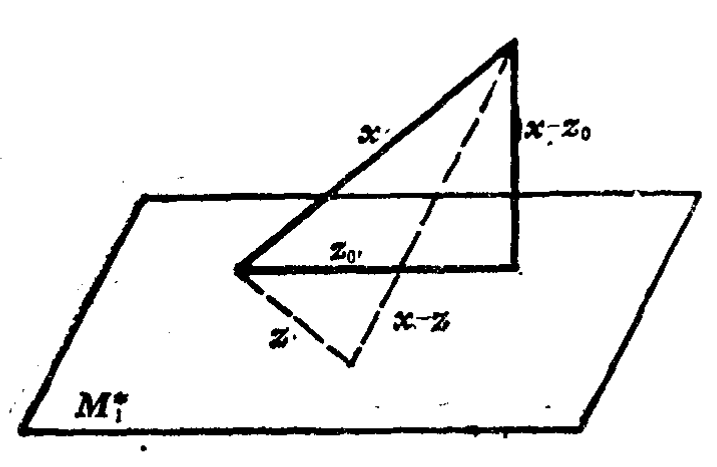
\includegraphics[width=0.4\textwidth]{正交投影.png}
            \caption{正交投影}
        \end{figure}

        由于$y(t)$是$z(t-\tau)$的无限线性组合，则$y(t)$和$z(t)$均在$M_1^*$中，根据正交投影定理，均方误差极小时，必有$r(t)-y(t)\perp M_1^*$，故有
        \[
        (r(t)-y(t),z(t-\lambda))=0\text{即}(r(t),z(t-\lambda))=(y(t),z(t-\lambda))
        \]

        则有
        \[
        R_{rz}(\lambda)=E\{r(t)z(t-\lambda)\}=E\{[\int_{-\infty}^\infty h(\tau)z(t-\tau)\d\tau]z(t-\lambda)\}=\int_0^\infty h(\tau)R_{zz}(\lambda-\tau)\d\tau
        \]

        此即为维纳-何甫（Wiener-Hopf）方程。

        对于功率谱密度可分解的情形，令
        \[
        q(\lambda)=\int_0^\infty h(\tau)R_{zz}(\lambda-\tau)\d\tau-R_{rz}(\lambda)
        \]

        则Wiener-Hopf方程要求$\forall\lambda\geqslant0,q(\lambda)=0$。对上式进行双边Laplace变换后得$Q(s)=H(s)R_{zz}(s)-R_{rz}(s)$。
        
        为了满足$q(\lambda)=0$，$Q(s)$必须没有极点在s左半平面。因此如果不加约束$H(s)$一般会在右边平面有极点，系统不具有因果性不可实现。因此需要要求$H(s)$在右半平面没有极点。

        对$R_{zz}(s)$进行谱分解，将极点和零点都在右半平面的与极点和零点都在左半平面的分解开，有
        \[
        R_{zz}(s)=R_{zz}(s)_R R_{zz}(s)_L
        \]

        代入Laplace变换中，并将后一项按极点位置进行部分分式分解，有
        \[
        Q(s)=R_{zz}(s)_R[H(s)R_{zz}(s)_L-\frac{R_{rz}(s)}{R_{zz}(s)_R}]=R_{zz}(s)_R\{H(s)R_{zz}(s)_L-[\frac{R_{rz}(s)}{R_{zz}(s)_R}]_{LP}-[\frac{R_{rz}(s)}{R_{zz}(s)_R}]_{RP}\}
        \]

        由于$Q(s)$在左半平面无极点，则有
        \[
        H(s)R_{zz}(s)_L-[\frac{R_{rz}(s)}{R_{zz}(s)_R}]_{LP}=0
        \]

        因此Wiener-Hopf方程的解为
        \[
        H(s)=\frac{1}{R_{zz}(s)_L}[\frac{R_{rz}(s)}{R_{zz}(s)_R}]_{LP}
        \]

        通过求解Wiener-Hopf方程，求出滤波器的最优传递函数，这种最优线性滤波称为维纳（Wiener）滤波。
    \subsection{最小方差控制律问题}
        以下研究单输入单输出线性定常离散系统的调节器问题，其中噪声是高斯平稳序列，具有有理功率谱密度。控制对象的差分方程为
        \[
        y(n)+a_1y(n-1)+\cdots+a_ky(n-k)=b_0u(n-l)+b_1u(n-l-1)+\cdots+b_k(n-l-k)+\lambda[e(n)+c_1e(n-1)+\cdots+c_ke(n-k)]
        \]

        利用$z^{-1}y(n)=y(n-1)$，将差分方程写成
        \[
        A(z)y(n)=B(z)u(n-l)+\lambda C(z)e(n)
        \]

        其中
        \[
        \begin{cases}
        A(z)=1+a_1z^{-1}+\cdots+a_kz^{-k}\\
        B(z)=b_0+b_1z^{-1}+\cdots+b_kz^{-k}\\
        A(z)=1+c_1z^{-1}+\cdots+c_kz^{-k}\\
        \end{cases}
        \]

        因此可以将随机干扰的影响等效成$v(n)=\lambda\dfrac{C(z)}{A(z)}e(n)$。

        若$A(z),B(z),C(z)$全部零点都在单位圆内，则输出为宽平稳随机序列，功谱密度为
        \[
        R_v(z)=\lambda^2\frac{C(z)C(z^{-1})}{A(z)A(z^{-1})},z=\e^{\j\omega}
        \]

        将$C(z)$部分分式分解后，等效干扰
        \[
        v(n)=\lambda[F(z)+z^{-l}\frac{G(z)}{A(z)}]e(n)
        \]

        则将输出方程写为
        \begin{align*}
        y(n+l)&=\frac{B(z)}{A(z)}u(n)+\lambda F(z)e(n+l)+\lambda\frac{G(z)}{A(z)}e(n)\\
        &=\lambda F(z)e(n+l)+[\frac{B(z)}{A(z)}-z^{-l}\frac{B(z)G(z)}{A(z)C(z)}]u(n)+\frac{G(z)}{C(z)}y(n)\\
        &=\lambda F(z)e(n+l)+\frac{B(z)}{C(z)}F(z)u(n)+\frac{G(z)}{C(z)}y(n)
        \end{align*}

        因此方差为
        \[
        E\{y^2(n+l)\}=E\{[\lambda F(z)e(n+l)]^2\}+E\{[\frac{B(z)}{C(z)}F(z)u(n)+\frac{G(z)}{C(z)}y(n)]^2\}
        \]

        为使方差最小，第二项应为零，即
        \[
        B(z)F(z)u(n)+G(z)y(n)=0
        \]

        最小方差控制律下系统输出的方差为
        \[
        J_{\min}=E\{y^2(n+l)\}=\lambda(1+f_1^2+\cdots+f_{l-1}^2)
        \]
\newpage
\section{状态估计}
    \paragraph{维纳滤波的不足之处}
    \begin{enumerate}
        \item 涉及平稳随机过程，对于非平稳随机过程很难应用；
        \item 方程求解过程困难；
        \item 应用计算机求解时，需要存储和处理大量数据，根据整个区间的数据得出滤波结果。
    \end{enumerate}
    \subsection{离散时间线性系统的Kalman滤波}
        对于离散系统
        \[
        \begin{cases}
        \bm{x}(n+1)&=\bm{\varPhi}(n+1,n)\bm{x}(n)+\bm{\theta}(n+1,n)\bm{u}(n)+\bm{\varGamma}(n+1,n)\bm{w}(n)\\
        \bm{y}(n)&=\bm{C}(n)\bm{x}(n)+\bm{D}(n)\bm{u}(n)+\bm{v}(n)\\
        \end{cases}
        \]
        
        根据已取得的一组序贯观测值$\mathscr{Y}(j)=\{\bm y(1),\bm y(2),\cdots,\bm y(j)\}$求出n时刻或区间的状态$\bm x(n)$的最优线性估计值$\bm{\hat x}(n|j)$，若状态估计误差$\bm{\tilde x}(n|j)=\bm x(n)-\bm{\hat x}(n|j)$，则最优线性估计值$\bm{\hat x}(n|j)$满足
        \begin{enumerate}
            \item 时观测序列$\mathscr{Y}(j)$的线性函数
            \item 是条件无偏的或无条件无偏的，即$E\{\bm{\hat x}(n|j)|\mathscr{Y}(j)\}=E\{\bm x(n)|\mathscr{Y}(j)\}$或$E\{\bm{\hat x}(n|j)\}=E\{\bm x(n)\}$
            \item 估计误差的方差最小，即$Var\{\bm{\tilde x}(n|j)\}$或$Var\{\bm{\tilde x}(n|j)|\mathscr{Y}(j)\}$最小。
        \end{enumerate}

        \paragraph{根据n与j的关系，状态估计问题分为}
        \begin{enumerate}
            \item $n>j$，则为预测或外推问题，根据现在时刻及以前的观测值区估计将来时刻的状态。
            \item $n=j$，则为滤波问题，根据现在时刻及以前获得的观测数据估计现在时刻的状态。
            \item $n<j$，则为平滑或内插问题，根据现在时刻及以前获得的观测数据估计以前某个时刻或区间的状态。
        \end{enumerate}

        假设$\bm w(n),\bm v(n)$为互不相关的零均值白噪声序列，其中
        \[
        Cov\{\bm w(k),\bm w(j)\}=\bm Q(k)\delta_{kj},Cov\{\bm v(k),\bm v(j)\}=\bm R(k)\delta_{kj}
        \]
        $\bm Q$为对称非负定阵，$R$为对称正定阵。$\bm x(0)$为随机向量且与$\bm{w}(n),\bm v(n)$独立。
        \subsubsection{一步预测估计}
            一个状态的最小方差线性估计，按投影定理解释，就是该状态向量在线性观测空间上的正交投影，根据投影定理的线性可知，状态估计也满足状态方程，则有
            \[
            \bm{\hat x}(n|n-1)=\bm{\varPhi}(n,n-1)\bm{\hat x}(n-1|n-1)+\hat E\{\bm{\varGamma}(n,n-1)\bm{w}(n-1)|\mathscr{Y}(n-1)\}=\bm{\varPhi}(n,n-1)\bm{\hat x}(n-1|n-1)
            \]

            则根据观测方程有
            \[
            \bm{\hat y}(n|n-1)=\bm{C}(n)\bm{\hat x}(n|n-1)
            \]

            观测误差
            \[
            \bm{\tilde y}(n|n-1)=\bm y(n)-\bm{\hat y}(n|n-1)=\bm C(n)[\bm x(n)-\bm{\hat x}(n|n-1)]+\bm v(n)
            \]

            按投影定理，最小方差估计误差$[\bm x(n)-\bm{\hat x}(n|n-1)]$与空间$\mathscr{Y}(n-1)$正交，$\bm v(n)$也与$\mathscr{Y}(n-1)$无关正交，因此偏差$\bm{\tilde y}(n|n-1)$也与$\mathscr{Y}(n-1)$正交。但$\bm{\tilde y}(n-1|n-2)$是在$\mathscr{Y}(n-1)$中，因此$\bm{\tilde y}(n|n-1)$和$\bm{\tilde y}(n-1|n-2)$正交，因此$\bm{\tilde y}(\cdot|\cdot)$为白噪声序列。

            由于$\bm{\tilde y}(\cdot|\cdot)$为白噪声序列，后来与先前无关，则可以用$\bm{\tilde y}(n|n-1)$作为获得的新信息对状态$\bm x(n)$的估计进行改善，即
            \[
            \bm{\hat x}(n|n)=\bm{\hat x}(n|n-1)+\bm K(n)\bm{\tilde y}(n|n-1)
            \]

            此即为最优线性滤波递推方程。式中$\bm K(n)$为Kalman滤波增益矩阵，需要根据误差方差达到极小来确定。
        \subsubsection{滤波增益矩阵}
            滤波估计误差为
            \begin{align*}
            \bm{\tilde x}(n|n)&=\bm x(n)-\bm{\hat x}(n|n)\\
            &=\bm x(n)-\bm{\hat x}(n|n-1)-\bm K(n)[\bm y(n)-\bm C(n)\bm{\hat x}(n|n-1)]\\
            &=\bm{\tilde x}(n|n-1)-\bm{K}(n)[\bm C(n)\bm{\tilde x}(n|n-1)+\bm v(n)]
            \end{align*}

            为使估计误差极小，则根据正交投影定理，$E\{\bm{\tilde x}(n|n)\bm y^T(n)\}=0$，则有
            \begin{align*}
            &E\{[\bm{\tilde x}(n|n-1)-\bm{K}(n)\bm C(n)\bm{\tilde x}(n|n-1)-\bm K(n)\bm v(n)][\bm C(n)\bm x(n)+\bm v(n)]^T\}\\
            &=E\{[\bm{\tilde x}(n|n-1)-\bm{K}(n)\bm C(n)\bm{\tilde x}(n|n-1)-\bm K(n)\bm v(n)]\\
            &\times[\bm C(n)\bm{\tilde x}(n|n-1)+\bm C(n)\bm{\hat x}(n|n-1)+\bm v(n)]^T\}=\bm 0                
            \end{align*}

            即
            \[
            E\{\bm{\tilde x}(n|n-1)\bm{\tilde x}^T(n|n-1)\bm C^T(n)-\bm{K}(n)\bm C(n)E\{\bm{\tilde x}(n|n-1)\bm{\tilde x}^T(n|n-1)\}\}\bm C^T(n)-\bm K(n)E\{\bm v(n)\bm v^T(n)\}=\bm 0
            \]

            令预测估计误差的方差$E\{\bm{\tilde x}(n|n-1)\bm{\tilde x}^T(n|n-1)\}=\bm P(n|n-1)$，则增益矩阵
            \[
            \bm K(n)=\bm P(n|n-1)\bm C^T(n)[\bm C(n)\bm P(n|n-1)\bm C^T(n)+\bm R(n)]^{-1}
            \]

            滤波估计误差的方差为
            \begin{align*}
            \bm P(n|n)&=E\{\bm{\tilde x}(n|n)\bm{\tilde x}^T(n|n)\}\\
            &=[I-\bm K(n)\bm C(n)]\bm P(n|n-1)[I-\bm K(n)\bm C(n)]^T+\bm K(n)\bm R(n)\bm K^T(n)\\
            &=[I-\bm K(n)\bm C(n)]\bm P(n|n-1)    
            \end{align*}

            从而滤波增益也可以写成$\bm K(n)=\bm P(n|n)\bm C^T(n)\bm R^{-1}(n)$。

            \begin{figure}[H]
                \centering
                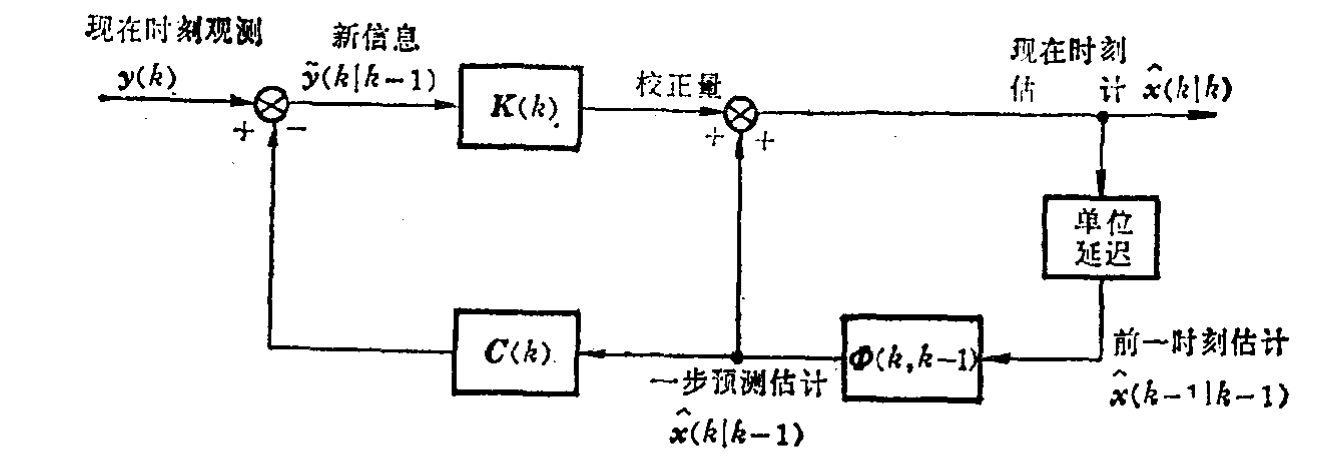
\includegraphics[width=0.6\textwidth]{离散Kalman结构图.png}
                \caption{离散Kalman滤波结构图}
            \end{figure}

            \begin{figure}[H]
                \centering
                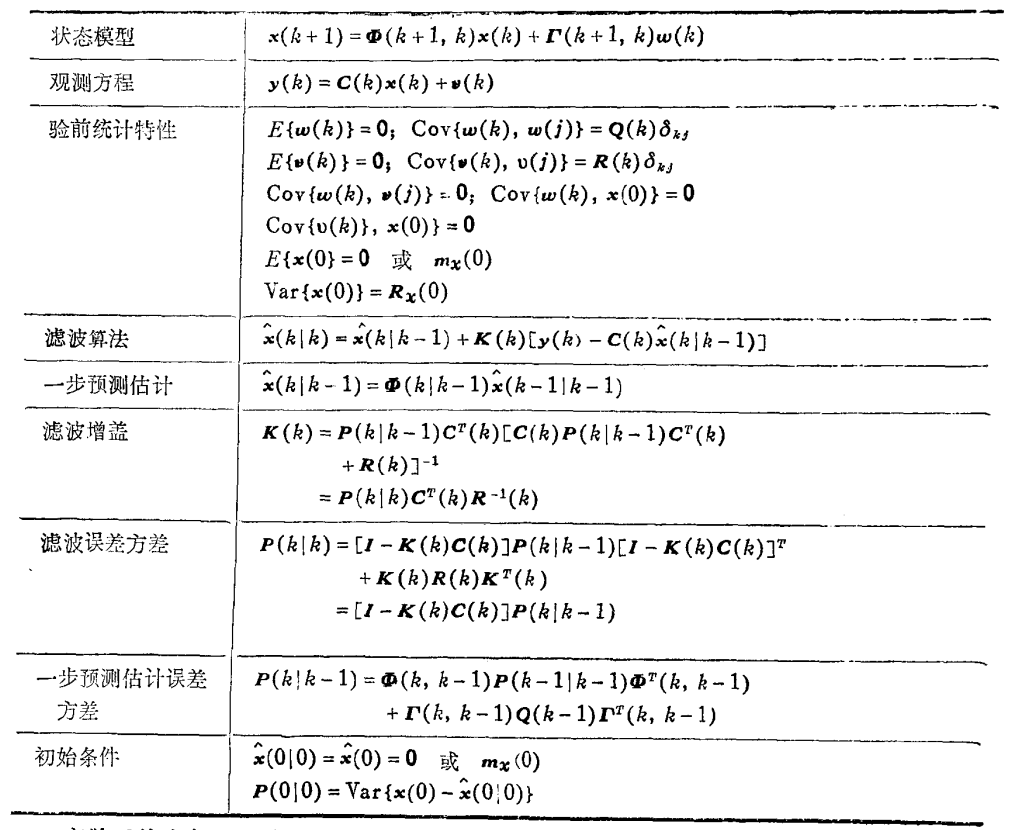
\includegraphics[width=0.7\textwidth]{离散Kalman总结.png}
                \caption{离散Kalman滤波算法}
            \end{figure}
        \subsubsection{一般情况下的Kalman滤波算法}
            \begin{enumerate}
                \item 系统的确定性输入$\bm u(n)\neq0$
                \item 观测方程存在确定性误差项$\bm z(n)$
                \item 随机输入$\bm w(n)$和观测噪声$\bm v(n)$均为均值不等于零的白噪声，且两者相关，即
                \[
                E\{\bm w(n)\}=\bm{m_w}(n),E\{\bm v(n)\}=\bm{m_v}(n),Cov\{\bm w(k),\bm(j)\}=\bm S(k)\delta_{kj}
                \]
            \end{enumerate}

            \paragraph{变换状态方程}\leavevmode

            将状态方程改写为
            \begin{align*}
            \bm{x}(n+1)&=\bm{\varPhi}(n+1,n)\bm{x}(n)+\bm{\theta}(n+1,n)\bm{u}(n)+\bm{\varGamma}(n+1,n)\bm{w}(n)\\
            &+\bm{J}(n)[\bm y(n)-\bm C(n)\bm x(n)-\bm z(n)-\bm v(n)]\\
            &=[\bm{\varPhi}(n+1,n)-\bm J(n)\bm C(n)]\bm x(n)+\bm{\theta}(n+1,n)\bm{u}(n)\\
            &+\bm J(n)[\bm y(n)-\bm z(n)]+[\bm{\varGamma}(n+1,n)\bm{w}(n)-\bm J(n)\bm v(n)]    
            \end{align*}

            记为
            \[
            \bm{x}(n+1)=\bm{\varPhi}^*(n+1,n)\bm x(n)+\bm{\theta}(n+1,n)\bm{u}(n)+\bm J(n)[\bm y(n)-\bm z(n)]+\bm{w}^*(n)
            \]

            其中$\bm{\varPhi}^*(n+1,n)=\bm{\varPhi}(n+1,n)-\bm J(n)\bm C(n),\bm{w}^*(n)=\bm{\varGamma}(n+1,n)\bm{w}(n)-\bm J(n)\bm v(n)$

            此时新的随机输入与观测噪声之间的协方差阵为
            \[
            Cov\{\bm w^*(n),\bm v(j)\}=Cov\{\bm\varGamma(n+1|n)\bm w(n),\bm v(j)\}-Cov\{\bm J(n)\bm v(n),\bm v(j)\}=[\bm\varGamma(n+1|n)\bm S(n)-\bm J(n)\bm R(n)]\delta_{nj}
            \]

            令上式等于零即可得
            \[
            \bm J(n)=\bm\varGamma(n+1|n)\bm S(n)\bm R^{-1}(n)
            \]

            \paragraph{导出随机向量偏差方程}\leavevmode

            由于观测数据$\bm y(n)$是确定性数据，则有
            \[
            \bm{m_x}(n+1)=\bm\varPhi^*(n+1,n)\bm{m_x}(n)+\bm\theta(n+1,n)\bm u(n)+\bm J(n)[\bm y(n)-\bm z(n)]+\bm{m_{w*}}(n)
            \]

            其中$\bm{m_{w*}}(n)=\bm\varGamma(n+1,n)\bm{m_w}(n)-\bm J(n)\bm{m_v}(n)$

            状态方程和上式相减得状态偏差方程
            \[
            \bm x^0(n+1)=\bm\varPhi^*(n+1,n)\bm x^0(k)+\bm w^{*0}(n)
            \]

            其中偏差向量$\bm x^0(n)=\bm x(n)-\bm{m_x}(n),\bm w^{*0}(n)=\bm w^*(n)-\bm{m_{w*}}(n)$

            观测方程的均值方程为$\bm{m_y}(n)=\bm C(n)\bm{m_x}(n)+\bm z(n)\bm{m_v}(n)$，作差得到观测偏差方程
            \[
            \bm y^0(n)=\bm C(n)\bm x^0(n)+\bm v^0(n)
            \]

            \paragraph{滤波算法的推广}\leavevmode

            \begin{figure}[H]
                \centering
                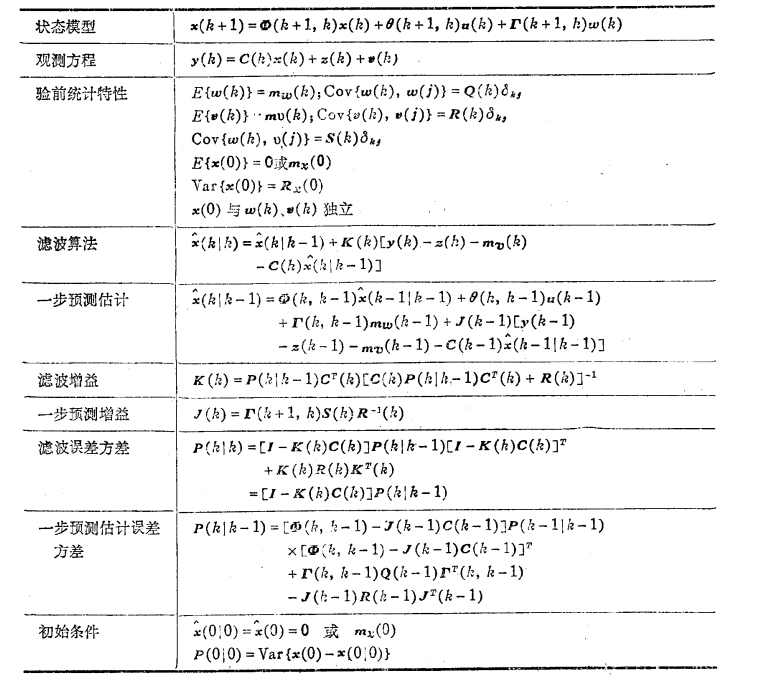
\includegraphics[width=0.7\textwidth]{离散Kalman一般情况.png}
                \caption{一般情况下的离散Kalman滤波算法}
            \end{figure}
        \subsubsection{有色噪声下的离散Kalman滤波}
            若过程噪声为有色噪声且观测噪声为白噪声，则可以用增广向量归一为噪声均是白噪声的形式；若过程噪声和观测噪声都是有色噪声，将产生有色噪声的线性系统与原状态方程化为白噪声输入的新的增广状态方程，再处理新的过程噪声为白噪声、观测噪声为有色噪声的情况。

            因此假定过程噪声为白噪声且观测噪声为有色噪声。系统的数学模型为
            \[
            \begin{cases}
            \bm{x}(n+1)=\bm{\varPhi}(n+1,n)\bm{x}(n)+\bm{\varGamma}(n+1,n)\bm{w}(n)\\
            \bm{y}(n+1)=\bm{C}(n+1)\bm{x}(n+1)+\bm{v}(n+1)\\
            \bm{v}(k+1)=\bm F(n+1,n)\bm v(n)+\bm H(n+1,n)\bm\xi(n)\\
            \end{cases}
            \]

            令$\bm z(n)=\bm y(n+1)-\bm F(n+1,n)\bm y(n)$，虽然能提供$\bm x(n)$信息，但是由于需要$n+1$时刻的观测数据$\bm y(n+1)$，只能延迟一步在$n+1$时刻被利用，是伪观测向量。代入数学模型得
            \[
            \bm{z}(n)=[\bm C(n+1)\bm\varPhi(n+1,n)-\bm F(n+1,n)\bm C(n)]\bm x(n)+[\bm C(n+1)\bm\varGamma(n+1,n)\bm w(n)+\bm H(n+1,n)\bm \xi(n)]
            \]

            令增广矩阵为
            \[
            \bm C^*(n)=\bm C(n+1)\bm\varPhi(n+1,n)-\bm F(n+1,n)\bm C(n),\bm v^*(n)=\bm C(n+1)\bm\varGamma(n+1,n)\bm w(n)+\bm H(n+1,n)\bm \xi(n)
            \]
            
            则状态方程可写为
            \[
            \bm z(n)=\bm C^*(n)\bm x(n)+\bm v^*(n)
            \]

            新观测方程中的噪声是零均值白噪声，且协方差
            \begin{align*}
            Cov\{\bm v^*(n),\bm v^*(j)\}=[\bm C(n+1)\bm\varGamma(n+1,n)\bm Q(n)\bm\varGamma^T(n+1,n)\bm C^T(n+1)\\
            +\bm H(n+1,n)\bm S(n)\bm H^T(n+1,n)]\delta_{nj}=\bm R^*(n)\delta_{nj}
            \end{align*}

            新观测方程的噪声和过程噪声相关，且互协方差为
            \[
            Cov\{\bm w(n),\bm v^*(j)\}=[\bm Q(n)\bm\varGamma^T(n+1,n)\bm C^T(n+1)]\delta_{nj}=\bm S^*(n)\delta_{nj}
            \]

            应用以前的滤波算法，按照状态方程和观测方程得到的一步预测估计$\bm{\hat x}(n|n+1)$和一步预测估计误差的方差$\bm P(n,n-1)$，实际上是原系统方程的状态估计$\bm{\hat x}(n|n)$和估计误差方差$\bm P(n|n)$。因此，按照伪观测数据$\mathscr{Z}(n-1)$求得的一部预测估计就是观测数据$\mathscr{Y}(n)$已知条件下的滤波估计。按照新观测方程求得的滤波估计是原方程的平滑估计。

            \begin{figure}[H]
                \centering
                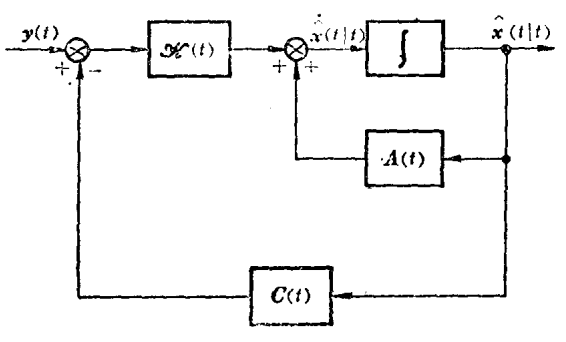
\includegraphics[width=0.5\textwidth]{连续Kalman结构图.png}
                \caption{连续Kalman滤波算法结构图}
            \end{figure}

            \begin{figure}[H]
                \centering
                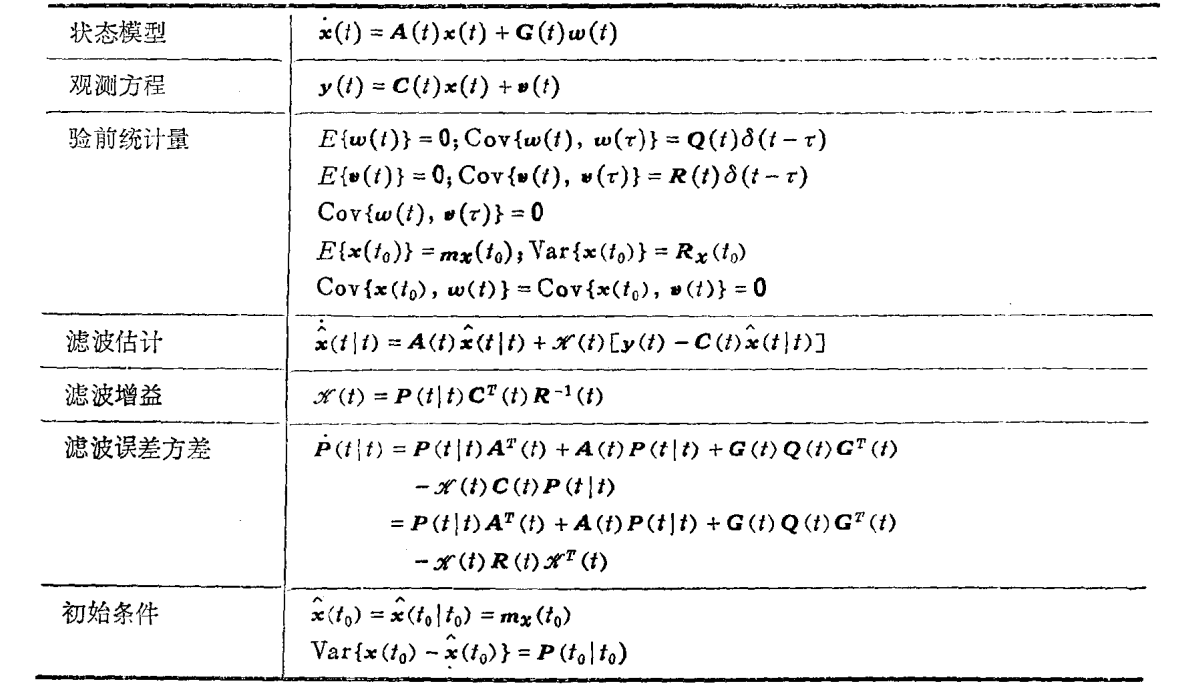
\includegraphics[width=0.7\textwidth]{连续Kalman总结.png}
                \caption{连续Kalman滤波算法}
            \end{figure}
    \subsection{连续时间线性系统的Kalman滤波}
        对于连续系统
        \[\begin{cases}
        \bm{\dot x}(t)=\bm{A}(t)\bm{x}(t)+\bm{B}(t)\bm{u}(t)+\bm{G}(t)\bm{w}(t)\\
        \bm{y}(t)=\bm{C}(t)\bm{x}(t)+\bm{D}(t)\bm{u}(t)+\bm{v}(t)\\
        \end{cases}\]
        根据时间区间$[t_0,t]$上获得的观测数据，求出$\tau$时刻的状态$\bm x(\tau)$的最优线性估计$\bm{\hat x(\tau/t)}$，是观测值的线性函数、无偏估计，且使估计误差的方差为极小。

        连续系统的估计问题也可以分为预测问题$\tau>t$、滤波问题$\tau=t$和平滑问题$\tau<t$。
        \subsubsection{滤波基本方程}
            假定$\bm w(t),\bm v(t)$为互不相关的零均值白噪声，且
            \[
            Cov\{\bm w(t),\bm w(\tau)\}=\bm Q(t)\delta(t-\tau),Cov\{\bm v(t),\bm v(\tau)\}=\bm R(t)\delta(t-\tau)
            \]         
            初始状态$\bm x(t_0)$为随机向量且与$\bm w(t),\bm v(t)$独立。

            令离散Kalman滤波算法中$n=t+\Delta t,n-1=t$，采样间隔为$\Delta t$，则式子变为
            \[\begin{cases}
            \bm{\hat x}(t+\Delta t|t+\Delta t)=\bm{\hat x}(t+\Delta t|t)+\bm K(t+\Delta t)[\bm y(t+\Delta t)-\bm C(t+\Delta t)\bm{\hat x}(t+\Delta t)]\\
            \bm{\hat x}(t+\Delta t|t)=\bm\varPhi(t+\Delta t,t)\bm{\hat x}(t|t)\\
            \bm K(n)=\bm K(t+\Delta t)=\bm P(t+\Delta t|t)\bm C^T(t+\Delta t)[\bm C(t+\Delta t)\times\bm P(t+\Delta t|t)\bm C^T(t+\Delta t)+\dfrac{\bm R(t+\Delta t)}{\Delta t}]^{-1}
            \end{cases}\]

            由前述知$\bm\varPhi(t+\Delta t,t)\bm I+\bm A(t)\Delta t$，则有
            \[
            \bm{\hat x}(t+\Delta t|t+\Delta t)=[\bm I+\bm A(t)\Delta t]\bm{\hat x}(t|t)+\bm K(t+\Delta t)[\bm y(t+\Delta t)-\bm C(t+\Delta t)\bm{\hat x}(t+\Delta t)]
            \]

            则滤波估计为
            \[
            \bm{\dot{\hat x}}(t|t)=\lim\limits_{\Delta t\rightarrow0}\frac{\bm{\hat x}(t+\Delta t|t+\Delta t)-\bm{\hat x}(t|t)}{\Delta t}=\bm A(t)\bm{\hat x}(t|t)+\lim\limits_{\Delta t\rightarrow0}\frac{\bm K(t+\Delta t)}{\Delta t}\times[\bm y(t)-\bm C(t)\bm{\hat x}(t|t)]
            \]

            由于$\lim\limits_{\Delta t\rightarrow0}\bm{\hat x}(t+\Delta t|t)=\lim\limits_{\Delta t\rightarrow 0}[\bm I+\bm A(t)\Delta t]\bm{\hat x}(t|t)$，则滤波估计方程为
            \[
            \bm{\dot{\hat x}}(t|t)=\bm A(t)\bm{\hat x}(t|t)+\mathscr{K}(t)[\bm y(t)-\bm C(t)\bm{\hat x}(t|t)]
            \]

            Kalman滤波增益阵为
            \[
            \mathscr{K}(t)=\lim\limits_{\Delta t\rightarrow0}\frac{\bm{K}(t+\Delta t)}{\Delta t}=\bm{P}(t|t)\bm C^T(t)\bm R^{-1}(t)
            \]

            估计误差的方差方程为
            \[
            \bm P(t+\Delta t|t)=\bm\varPhi(t+\Delta t,t)\bm P(t|t)\bm\varPhi^T(t+\Delta t,t)+\bm\varGamma(t+\Delta t,t)\frac{\bm Q(t)}{\Delta t}\bm\varGamma(t+\Delta t,t)
            \]

            由于$\bm\varGamma(t+\Delta t,t)=\bm\varPhi(t+\Delta t,t)\bm G(t)\Delta t=[\bm I+\bm A(t)]\bm G(t)\Delta t=\bm G(t)\Delta t$

            代入可得
            \[
            \bm P(t+\Delta t|t)=\bm P(t|t)+\bm P(t|t)\bm A^T(T)\Delta t+\bm A(t)\bm P(t|t)\Delta t+\bm A(t)\bm P(t|t)\bm A^T(t)(\Delta t)^2+\bm G(t)\bm Q(t)\bm G^T(t)\Delta t
            \]

            因此$\lim\limits_{\Delta t\rightarrow0}\bm P(t+\Delta t|t)=\bm P(t|t)$

            于是有
            \begin{align*}
            \bm{\dot P}(t|t)&=\lim\limits_{\Delta t\rightarrow 0}\frac{\bm P(t+\Delta t|t+\Delta t)-\bm P(t|t)}{\Delta t}\\
            &=\lim\limits_{\Delta t\rightarrow 0}\frac{\bm P(t+\Delta t|t)-\bm K(t+\Delta t)\bm C(t+\Delta t)\bm P(t+\Delta t|t)-\bm P(t|t)}{\Delta t}\\
            &=\bm P(t|t)\bm A^T(t)+\bm A(t)\bm P(t|t)+\bm G(t)\bm Q(t)\bm G^T(t)-\lim\limits_{\Delta t\rightarrow 0}\frac{\bm K(t+\Delta t)\bm C(t+\Delta t)\bm P(t+\Delta t|t)}{\Delta t}    
            \end{align*}

            利用Kalman滤波增益阵可得滤波估计误差的方差满足Riccati微分方程
            \[
            \bm{\dot P}(t|t)=\bm P(t|t)\bm A^T(t)+\bm A(t)\bm P(t|t)+\bm G(t)\bm Q(t)\bm G^T(t)-\mathscr{K}(t)\bm C(t)\bm P(t|t)
            \]

            书114总结和方框图

        \subsubsection{预测估计基本方程}
            由状态方程可得
            \[
            \bm x(t_2)=\bm\varPhi(t_2,t_1)\bm x(t_1)+\int_{t_1}^{t_2}\bm\varPhi(t_2,\tau)\bm G(\tau)\bm w(\tau)\d\tau
            \]

            根据正交投影定理，当获得观测数据$\mathscr{Y}(t_1)$后，状态的预测估计
            \[
            \bm{\hat x}(t_2|t_1)=\bm\varPhi(t_2,t_1)\bm{\hat x}(t_1|t_1)+\hat E\int_{t_1}^{t_2}\bm\varPhi(t_2,\tau)\bm G(\tau)\bm w(\tau)\d\tau=\bm\varPhi(t_2,t_1)\bm{\hat x}(t_1|t_1)
            \]
        \subsubsection{一般情况下的Kalman滤波算法}
            \[\begin{cases}
            \bm{\dot x}(t)=\bm{A}(t)\bm{x}(t)+\bm{B}(t)\bm{u}(t)+\bm{G}(t)\bm{w}(t)\\
            \bm{y}(t)=\bm{C}(t)\bm{x}(t)+\bm{z}(t)+\bm{v}(t)\\
            \end{cases}\]

            $\bm z(t)$为确定性误差，白噪声$\bm w(t),\bm v(t)$均值均不为零且相关，且
            \[
            R_w(t,\tau)=\bm Q(t)\delta(t-\tau),R_v(t,\tau)=\bm R(t)\delta(t-\tau),R_{wv}(t,\tau)=\bm S(t)\delta(t-\tau)
            \]
            
            由连续离散化关系
            \[
            \bm Q(n)=\frac{\bm Q(t+\Delta t)}{\Delta t}\qquad\bm R(n)=\frac{\bm R(t+\Delta t)}{\Delta t}\qquad\bm S(n)=\frac{\bm S(t+\Delta t)}{\Delta t}
            \]

            以及渐进相等关系
            \[
            \bm\varPhi(t+\Delta t,t)=\bm I+\bm A(t)\Delta t,\bm\varGamma(t+\Delta t,t)=\bm G(t)\Delta t,\bm\theta(t+\Delta t,t)=\bm B(t)\Delta t
            \]

            代入离散滤波方程得连续Kalman滤波基本方程为
            \[
            \bm{\dot{\hat x}}(t|t)=\bm A(t)\bm{\hat x}(t|t)+\bm B(t)\bm u(t)+\bm G(t)\bm{m_w}(t)+\mathscr{K}(t)[\bm y(t)-\bm z(t)-\bm{m_v}(t)-\bm C(t)\bm{\hat x}(t|t)]
            \]

            \[
            \mathscr{K}(t)=[\bm{P}(t|t)\bm C^T(t)+\bm G(t)\bm S(t)]\bm R^{-1}(t)
            \]
            
            \[
            \bm{\dot P}(t|t)=\bm P(t|t)\bm A^T(t)+\bm A(t)\bm P(t|t)+\bm G(t)\bm Q(t)\bm G^T(t)-\mathscr{K}(t)\bm C(t)\mathscr{K}^T(t)
            \]    
            
            且初值条件为$\bm{\hat x}(t_0|t_0)=\bm{m_x}(t_0),\bm P(t_0|t_0)=\bm{R_x}(t_0)$
        \subsubsection{有声噪声情况下的连续Kalman滤波}
            和离散情况相同，下面只考虑观测噪声为有色噪声、过程噪声为白噪声，且有色噪声是白噪声激励一个线性系统后的输出的情况。系统的数学模型为
            \[\begin{cases}
            \bm{\dot x}(t)=\bm{A}(t)\bm{x}(t)+\bm{G}(t)\bm{w}(t)\\
            \bm{y}(t)=\bm{C}(t)\bm{x}(t)+\bm{v}(t)\\
            \bm{\dot v}(t)=\bm F(t)\bm v(t)+\bm H(t)\bm\xi(t)\\
            \end{cases}\]

            $\bm w(t),\bm\xi(t)$都是零均值白噪声且互不相关，$R_w(t,\tau)=\bm Q(t)\delta(t-\tau),R_\xi(t,\tau)=\bm S(t)\delta(t-\tau)$

            仍采用变换观测方程的方法，令$\bm z(t)=\bm{\dot y}(t)-\bm F(t)\bm y(t)$，且令
            \[
            \begin{cases}
            \bm C^*(t)=\bm C(t)\bm A(t)+\dot{\bm C}(t)-\bm F(t)\bm C(t)\\
            \bm v^*(t)=\bm C(t)\bm G(t)\bm w(t)+\bm H(t)\bm\xi(t)\\
            \end{cases}
            \]

            且增广阵的自协方差和互协方差为
            \[
            \bm R_{v*}(t,\tau)=[\bm C(t)\bm G(t)\bm Q(t)\bm G^T(t)\bm C^T(t)+\bm H(t)\bm S(t)\bm H^T(t)]\delta(t-\tau),\bm R_{wv*}(t,\tau)=[\bm Q(t)\bm G^T(t)\bm C^T(t)]\delta(t-\tau)
            \]

            基本滤波公式为
            \[
            \bm{\dot{\hat x}}(t|t)=\bm A(t)\bm{\hat x}(t|t)+\mathscr{K}(t)\{\bm{\dot y}(t)-\bm F(t)\bm{y}(t)-[\bm C(t)\bm A(t)+\dot{\bm C}(t)-\bm F(t)\bm C(t)]\bm{\hat x}(t|t)\}
            \]

            \begin{align*}
            \mathscr{K}(t)=\{\bm{P}(t|t)[\bm C(t)\bm A(t)+\dot{\bm C}(t)-\bm F(t)\bm C(t)]^T+\bm G(t)\bm Q(t)\bm G^T(t)\bm C^T(t)\}\\
            \{\bm C(t)\bm G(t)\bm Q(t)\bm G^T(t)\bm C^T(t)+\bm H(t)\bm S(t)\bm H^T(t)\}^{-1}
            \end{align*}
            
            \begin{align*}
            \bm{\dot P}(t|t)&=\bm P(t|t)\bm A^T(t)+\bm A(t)\bm P(t|t)+\bm G(t)\bm Q(t)\bm G^T(t)\\
            &-\mathscr{K}(t)\{\bm C(t)\bm G(t)\bm Q(t)\bm G^T(t)\bm C^T(t)+\bm H(t)\bm S(t)\bm H^T(t)\}\mathscr{K}^T(t)
            \end{align*}

            加入观测从$t_0$开始，在$t_0$时就能进行估计，因为$\bm y(t_0)=\bm C(t_0)\bm x(t_0)+\bm v(t_0)$，因此线性最小方差估计是$\bm y(t_0)$的线性无偏函数，且具有最小估计误差方差。设$\bm{\hat x}(t_0|t_0)=\bm M+\bm{Ny}(t_0)$，则
            \[
            E\{\bm{\hat x}(t_0|t_0)\}=\bm M+\bm N E\{\bm y(t_0)\}=E\{\bm x(t_0)\}
            \]

            则$\bm M=E\{\bm x\}(t_0)-\bm NE\{\bm y(t_0)\}$

            再根据最小方差要求，估计误差向量与空间$\mathscr{Y}(t_0)$正交，则有
            \[
            Cov\{[\bm x(t_0)-\bm{\hat x}(t_0|t_0)],\bm y(t_0)\}=Cov\{\bm x(t_0),\bm y(t_0)\}-\bm NVar\{\bm y(t_0)\}=0
            \]

            则$\bm N=Cov\{\bm x(t_0),\bm y(t_0)\}[Var\{\bm y(t_0)\}]^{-1}$

            因此$\bm x(t_0)$的线性最小方差估计为
            \[
            \bm{\hat x}(t_0|t_0)=\bm{m_x}(t_0)+\bm{R_x}(t_0)\bm C^T(t_0)[\bm C(t_0)\bm{R_x}(t_0)\bm C^T(t_0)+Var\{\bm v(t_0)\}]^{-1}[\bm y(t_0)-\bm C(t_0)\bm{m_x}(t_0)]
            \]

            初值估计误差的方差为
            \begin{align*}
            \bm P(t_0|t_0)&=E\{[\bm x(t_0)-\bm{\hat x}(t_0|t_0)][\bm x(t_0)-\bm{\hat x}(t_0|t_0)]^T\}\\
            &=\bm{R_x}(t_0)-\bm{R_x}(t_0)\bm C^T(t_0)[\bm C(t_0)\bm{R_x}(t_0)\bm C^T(t_0)+Var\{\bm v(t_0)\}]^{-1}\bm C(t_0)\bm{R_x}(t_0)
            \end{align*}
        \subsubsection{平稳Kalman滤波}
            当系统是线性定常的，过程噪声和观测噪声是宽平稳的（即$\bm Q,\bm R$非时变），且两者互不相关，观测很早就开始，那么系统的过程是平稳的，状态估计问题也变成平稳问题，可以忽略滤波器的瞬变过程，$\bm{\dot P}(t|t)=0$，方差微分Riccati方程变成代数方程
            \[
            \bm 0=\bm{PA}^T+\bm{AP}+\bm{GQG}^T-\mathscr{K}\bm R\mathscr{K}^T
            \]

            且增益矩阵也为常值$\mathscr{K}=\bm{PC}^T\bm R^{-1}$，滤波方程变为
            \[
            \bm{\dot{\hat x}}=\bm A\bm{\hat x}(t)+\mathscr{K}[\bm y(t)-\bm C\bm{\hat x}(t)]
            \]

            此时平稳滤波估计问题和维纳-何甫方程在频域的求解结果一致，此时滤波器即是维纳滤波器，此时卡尔曼算法和维纳算法是等价的。
    \subsection{状态估计问题和控制问题的对偶关系}
        对偶原理：求解一个线性系统的最小方差线性估计问题，等效于求解该系统的确定性对偶系统的线性最优控制问题。

        \[\begin{cases}
        \bm{\dot x}(t)=\bm{A}(t)\bm{x}(t)+\bm{G}(t)\bm{w}(t)\\
        \bm{y}(t)=\bm{C}(t)\bm{x}(t)+\bm{v}(t)\\
        \end{cases}\]

        在获得观测数据$\mathscr{Y}(t_1)$后，若要求得$\bm  a^T\bm x(t_1)$的滤波估计$\bm a^T\bm{\hat x}(t_1)$，能使误差的方差最小且线性无偏，则可以采用如下形式
        \[
        \bm a^T\bm{\hat x}(t_1)=\int_{t_0}^{t_1}\bm u^T(t)\bm y(t)\d t+\bm b^T\bm{m_x}(t_0)
        \]

        因此求最优估计问题实际上是求取$\bm u^T(t),\bm b^T$，使得性能指标$J=Var[\bm a^T\bm x(t_1)-\bm a^T\bm{\hat x}(t_1)]$达到最小。

        源系统的对偶系统的状态方程为
        \[
        \bm{\dot z}(t)=-\bm A^T(t)\bm z(t)+\bm C^T(t)\bm u(t)
        \]

        边界条件为$\bm z(t_1)=\bm a$，选择$\bm b=\bm z(t_0)$，使得估计无偏，则性能指标可以写为
        \[
        J=\bm z^T(t_0)\bm{R_{x*}}(t_0)\bm z(t_0)+\int_{t_0}^{t_1}[\bm z^T(t)\bm Q^*(t)\bm z(t)+\bm u^T(t)\bm R(t)\bm u(t)]\d t
        \]

        其中$\bm{R_{x*}}(t_0)=\bm{R_x}(t_0)-\bm{m_x}(t_0)\bm{m_x}^T(t_0),\bm Q^*(t)=\bm G(t)\bm Q(t)\bm G^T(t)$

        为了使最优控制与标准形式相同，采用逆时间$t^0=T-t$，则状态方程为
        \[
        \bm{\dot z}(t^0)=\bm A^T(t^0)\bm z(t^0)-\bm C^T(t^0)\bm u(t^0)
        \]

        初始条件为$\bm z(t_1^0)=\bm a$

        二次型性能指标为
        \[
        J=\bm z^T(t_0^0)\bm{R_{x*}}(t_0^0)\bm z(t_0^0)+\int_{t_1^0}^{t_0^0}[\bm z^T(t^0)\bm Q^*(t^0)\bm z(t^0)+\bm u^T(t^0)\bm R(t^0)\bm u(t^0)]\d t^0
        \]
    \subsection{Kalman滤波器的性能分析}
        \subsubsection{稳定性}
            稳定性：线性系统时间充分长后，$\bm{\hat x}(n|n)$将不再依赖于初值选取，有界输入对应有界估计，同时$\bm P(n|n)$亦渐进不依赖于初值方差阵的选取。
            
            线性系统的状态方程可写为
            \begin{align*}
            \bm{\hat x(n)}&=\bm\varPsi(n,n-1)\bm{\hat x}(n-1)+\bm K(n)\bm y(n)\\
            \bm{\dot{\hat x}}(n)&=\bm A_f(t)\bm{\hat x}(t)+\mathscr{K}(t)\bm y(t)\\
            \end{align*}

            则系统的状态转移矩阵$\bm\varPsi(n,n-1)=\bm\varPhi(n,n-1)-\bm K(n)\bm C(n)\bm\varPhi(n,n-1)$，系统矩阵$\bm A_f(t)=\bm A(t)-\mathscr{K}(t)\bm C(t)$。滤波稳定性即是上述两个方程的解的Lyapunov稳定性。

            随机系统滤波稳定性的充分条件：系统是一致完全能控或一致完全能观，则最优滤波是大范围一致渐进稳定的。

            离散系统的滤波误差方差在$k\geqslant 2N$时满足
            \[
            \frac{\alpha}{1+(n\beta)^2}\bm I\leqslant\bm P(n|n)\leqslant\frac{1+(n\beta)^2}{\alpha}\bm I
            \]

            连续系统的滤波误差方差在$t\geqslant t_0+\Delta t$时满足
            \[
            \frac{\alpha}{1+(n\beta)^2}\bm I\leqslant\bm P(t|t)\leqslant\frac{1+(n\beta)^2}{\alpha}\bm I
            \]

            推论：若系统是一致完全能控和一致完全能观的，且$\bm P_0^{(1)}$和$\bm P_0^{(2)}$是两个不同的初始估计误差的方差，则存在常数$c_3,c_4>0$，使得对所有$n\geqslant0$或$t\geqslant t_0$，有
            \[
            \|\bm P^{(2)}(n)-\bm P^{(1)}(n)\|\leqslant c_4\e^{-c_3n}\|\bm P_0^{(2)}-\bm P_0^{(1)}\|
            \]

            \[
            \|\bm P^{(2)}(t)-\bm P^{(1)}(t)\|\leqslant c_4\e^{-c_3(t-t_0)}\|\bm P_0^{(2)}-\bm P_0^{(1)}\|
            \]
        \subsubsection{模型误差}
            真实系统模型为
            \[\begin{cases}
            \bm{\dot x}(t)=\bm{A}(t)\bm{x}(t)+\bm{G}(t)\bm{w}(t)\\
            \bm{y}(t)=\bm{C}(t)\bm{x}(t)+\bm{v}(t)\\
            \end{cases}\]
            
            但是Kalman滤波时却使用了不精确的模型
            \[\begin{cases}
            \bm{\dot{\bar x}}(t)=\bar{\bm A}(t)\bm{\bar x}(t)+\bar{\bm G}(t)\bm{\bar w}(t)\\
            \bm{\bar y}(t)=\bar{\bm C}(t)\bm{\bar x}(t)+\bm{\bar v}(t)\\
            \end{cases}\]

            则实际估计误差和误差的方差满足
            \[
            \bm{\dot{\tilde x}_a}(t)=[\bar{\bm A}(t)-\bar{\mathscr{K}}(t)\bar{\bm C}(t)]\bm{\tilde x_a}(t)+[\Delta\bm A(t)-\bar{\mathscr{K}}(t)\Delta\bm C(t)]\bm x(t)+\bm G(t)\bm w(t)-\bar{\mathscr{K}}(t)\bm v(t)
            \]

            \begin{align*}
            \bm{\dot P_a}(t)&=[\bar{\bm A}(t)-\bar{\mathscr{K}}(t)\bar{\bm C}(t)]\bm{P_a}(t)+\bm{P_a}(t)[\bar{\bm A}(t)-\bar{\mathscr{K}}(t)\bar{\bm C}(t)]^T\\
            &+[\Delta\bm A(t)\bar{\mathscr{K}}(t)\Delta\bm C(t)]\bm{P_{x\tilde x_a}}(t)+\bm{P_{x\tilde x_a}}(t)[\Delta\bm A(t)\bar{\mathscr{K}}(t)\Delta\bm C(t)]^T\\
            &+\bm G(t)\bm Q(t)\bm G^T(t)+\bar{\mathscr{K}}(t)\bm R(t)\bar{\mathscr{K}}^T(t)
            \end{align*}

            只有当$\Delta\bm A=\Delta\bm C=\bm 0$时，估计是无偏的。
        \subsubsection{发散}
            当观测数据逐渐增多时，滤波估计应越来越准确，方差应逐渐趋于零或稳态值，但实际中，真正的实际误差有时却会大得不能允许甚至出现趋向无穷大的现象。
            
            产生发散的主要原因是：(1)系统模型不精确；(2)计算过程中舍入误差引起的数值计算不稳定。

            克服滤波发散可以：(1)使用非线性模型；(2)调整滤波算法；(3)或改进数值计算的精度。
            
            可以使用限定下界法限定增益矩阵（或误差方差等）减小的最小值，不会随时间增加趋于零。

            \paragraph{次优滤波器}\leavevmode

            可以使用次优滤波器，如衰减记忆滤波或限定记忆滤波，增强新观测数据的作用，减小前观测数据的影响。

            \begin{itemize}
                \item 衰减记忆滤波：将$n+1$时量测噪声协方差增加为$R_2(n+1)\e^{\sum_{n+1}^Nc_i}$，离N越远权重越大。将$n+1$时刻过程噪声协方差增加为$R_1(n+1)\e^{\sum_{n+1}^Nc_i}$，$P(n_0|n_0)$增加为$P(n_0|n_0)\e^{\sum_{0}^Nc_i}$，这是指数衰减记忆滤波，滤波算法为
                \[
                \hat x(n+1|n+1)=\hat x(n+1|n)+K(n+1)[y(n+1)-C\hat x(n+1|n)]
                \]

                \[
                P(n+1|n+1)=P(n+1|n)C^T[CP(n+1|n)C^T+R_2]^{-1}
                \]

                滤波增益为$K(n+1)=P(n+1|n)C^T[CP(n+1|n)C^T+R_2]^{-1}$

                将衰减因子由$\e^{c_i}$改为$s$则为几何极数衰减记忆滤波。
                \item 限定记忆滤波：$\xi(n)=0$，使用N个量估计当前状态，状态空间为$\mathscr{Y}(n)=\{y(n_0),\cdots,y(d),y(d+1),\cdots,y(n-1),y(n)\}$，则滤波算法为
                \begin{align*}
                \hat x^N(n|n)&=\varPhi(n,n-1)\hat x^N(n-1|n-1)+K(n)[y(n)-C(n)\varPhi(n,n-1)\hat x^N(n-1|n-1)]\\
                &-\bar K(n)[y(d)-C(d)\varPhi(d,n)\varPhi(n,n-1)\hat x^N(n-1|n-1)]    
                \end{align*}

                \begin{align*}
                P^N(n|n)&=[\varPhi^T(n,n-1)P^N(n-1|n-1)^{-1}\varPhi(n,n-1)+C(n)^TR_2^T(n)C(n)\\
                &-\varPhi^T(d,n)C^T(d)R_2^{-1}(d)C(d)\varPhi(d,n)]^{-1}
                \end{align*}

                其中卡尔曼滤波增益为$K(n|n)=P^N(n|n)C^T(n)R_2^{-1}(n),\bar K(n|n)=P^N(n|n)\varPhi^T(d,n)C^T(d)R_2^{-1}(d)$。
            \end{itemize}
            

            
            \paragraph{自适应滤波}\leavevmode

            为了随时根据观测值修改系统数学模型，可以使用自适应滤波，将系统辨识和状态估计结合起来，不断观测不断估计系统模型的不确定参数，对系统模型随时修正，不断进行状态估计。

            \paragraph{平方根滤波算法}\leavevmode

            理论依据：若$\bm B$是任意实矩阵，则$\bm A=\bm B^T\bm B$是对称非负定的；反之，若$\bm A$是非负定的对称阵，则可以找到$\bm B$使得$\bm B^T\bm B=\bm A$。
            
            在Kalman滤波算法中，将估计误差方差分解如下
            \[
            \bm P(n|n)=\bm S^T(n|n)\bm S(n|n)
            \]

            其中$\bm S=\sqrt{\bm P}$，则此时能保证$\bm P$是对称非负定的，消除计算误差。
\end{document}